\chapter{Understanding the effect of IAC on looking up information}

\begin{mynote}
\subsubsection{Chapter outline}
The previous chapter demonstrated that for an expenses task, people have to copy data from multiple sources that differ in terms of their IAC. This chapter describes two studies that explore the extent to which IACs influence strategies, speed and accuracy. 

Study 3 tests how IAC affects switching behaviour when copying from one source. It tested whether the effect of IAC on copying colours, as shown in previous studies, extends to copying numbers. Study 4 tests how IAC affects switching behaviour when information for one entry task has to be collected from multiple sources.
Together these studies intend to show that IAC affects how people switch between entering and looking up information.

\end{mynote}

 
\section{Study 3: Copying numbers from one source}\label{ch:Study2}
\subsection{Introduction}
Study 1 and 2 illustrated that people had to retrieve and copy data from multiple sources with varying information access costs (IAC). People were not always able to look at the data source while entering data, and information sometimes had to be briefly kept in memory before people could enter it.
In this situation, people have various options: they can decide to keep going back to the target source, reduce their memory load by writing it down, or keep as much of it in memory. Participants in Study 1 explained they tried to do it in the quickest way possible, and preferred to keep data in memory as this was often a faster strategy than writing it down, printing it out, or going back and forth between the source and the input window.

This is in line with previous lab studies, which showed that as the cost to access information increases, people increasingly rely on the information in their head rather than the information in the environment \citep[e.g.][]{Gray2006, Morgan2009}. People look at the target source longer before copying anything, but after one look, they do enter more items in one sequence before looking back. 

\citet{Gray2004} conducted a study where people had to copy over VCR programming information. Participants either had permanent access to the information, the information was covered by a grey box which could be uncovered by hovering over it with the cursor, or they were explicitly instructed and trained before the trial to memorise the information. The people in the latter condition were more accurate than the other conditions in entering the information. This shows that a deeper encoding of the information in memory makes people more accurate in entering the information. 

In later studies that further explored the effect of access costs on use of memory, the Blocks World Task (BWT) was used as a task paradigm, which requires people to copy a 3x3 grid of coloured blocks. In these studies, participants relied more on memory as the cost to access the target window increased. In one study, this memory-based strategy made participants better able to resume after interruptions by copying more blocks before having to revisit the target window \citep{Morgan2009}. Looking at overall task performance overall however, they did make more errors overall and took considerably longer to complete the task. In a later paper, the researchers reflected that the coloured blocks participants had to copy may have been too demanding to memorise \citep{Waldron2011}. This abstract visuo-spatial information did not bear any meaning to the participant, in contrast with the VCR programming information used in \citet{Gray2004} which is more familiar and easy to memorise. This suggests that the type of information to copy influences the effect that IAC might have on task performance, though the studies differed in task paradigm making it hard to compare their findings: in \citet{Gray2004} people were explicitly instructed to memorise the information and conducted a test prior to a trial during which they had to fill in the information, and could not continue until they had stated everything correctly. This ensured that people had the information well-memorised before they started the experimental trial. In the Blocks World Task studies, participants were not given this training or instruction.

Rather than training participants to memorise the information, \citet{Soboczenski2013} used an alternative approach to motivate people to encode the information more deeply. They conducted two studies where people had to transcribe text and numbers that were presented either in a black font colour or a harder-to-read grey font colour. Participants made fewer data transcription errors if data was shown in the harder-to-read font colour, both for transcribing text and numbers. In line with \citet{Gray2004}, these studies showed that when people do make the effort to more deeply encode information in a copying task, it can improve their accuracy.

In order to design data entry interfaces that support how people enter expenses from information sources with varying IACs, it is important to understand how these differences in IAC affect strategy and task performance. Relying on information in the head over information in the world can make it more likely for people to make errors in a copying task\citep{Morgan2009}, though other studies have shown that a deeper encoding of information can also improve accuracy if memorised well \citep{Gray2004, Soboczenski2013}. 

The study reported in this chapter replicates the BWT study, by using both coloured and numbered blocks.The purpose of this study is to see whether the effect on IAC on people's strategies and performance, as reported in previous BWT studies, holds when people have to copy numbers instead of colours.

It is expected that the effect of IAC on strategy will be similar and that an increase in IAC will encourage people to adopt a more memory-based strategy.  However, the expectation is that numbers are easier to memorise and people will be able to memorise more items. Furthermore, based on previous findings that a deeper encoding of numbers in memory can reduce errors, it is expected that an increased IAC will improve accuracy for copying numbers.


\subsection{Method}
\subsubsection{Participants}
Fourty-two participants (eight male) were recruited from the UCL Psychology Subject Pool. Ages ranged from 18 to 52 with a mean age of 22.38 (SD = 7.45). Participants received course credit or \pounds3.75 as a compensation for taking part in the study.

\subsubsection{Design}
A mixed design was used with two independent variables: IAC and block type.
The between-participants variable was the level of IAC which had three levels. If the IAC was Low, the target pattern was permanently visible. In the Medium and High IAC conditions, the target pattern was covered with a grey mask, and could only be uncovered by moving the mouse cursor over the window. The mask reappeared as soon as the cursor left the window. In the High IAC condition, there was an additional 1-second delay to uncover the mask. This delay time was used in previous BWT studies where it showed to have a significant effect on task strategies and performance \citep{Gray2006, Morgan2009, Waldron2007}.
The within-participants variable was the block type to be copied, which was either coloured or numbered blocks. The order was counter-balanced across participants.

The dependent variables are listed in Table \ref{table:ch4_dvs}. The primary focus is on the measures of the first visit, as participants do not have any information yet on the target pattern. On subsequent visits, they may already have partial information in their head from previous visits. Therefore, the items copied after the first visit is believed to be the most 'sensitive measure of performance' \citep{Janssen2012}. 
Two dependent variables were used to measure accuracy. Incorrectly placed blocks measured instances where a participant initially placed a block in the incorrect place, but then moved this to the correct place prior to submitting the pattern. Incorrectly submitted trials measured instances where the participant had finished copying a pattern and clicked the Submit button, but the pattern was incorrect.

\begin{table}[htp]
\centering
    \begin{tabular}{  l }
    \hline
    \textbf{ Strategy measures} \\  
    Number of visits to target window  \\ 
    Visit duration of first visit (s)  \\
    Average duration of visits (s) \\
    Number of blocks copied after first visit \\
    Number of blocks copied correctly after first visit 
    
    \vspace{10pt} \\
    
\textbf{Global task performance measures} \\ 
Number of incorrectly placed blocks (per trial) \\
Number of incorrectly submitted trials (per experiment block) \\
Trial completion time incl. and excl. lockout (s) \\ \hline
    \end{tabular}
    \caption[Study 3 dependent variables]{Dependent variables used in the study.}
    \label{table:ch4_dvs}
\end{table}

\subsubsection{Materials}
\begin{figure}[]
\begin{center}

\begin{subfigure}[b]{\textwidth}
\centerline{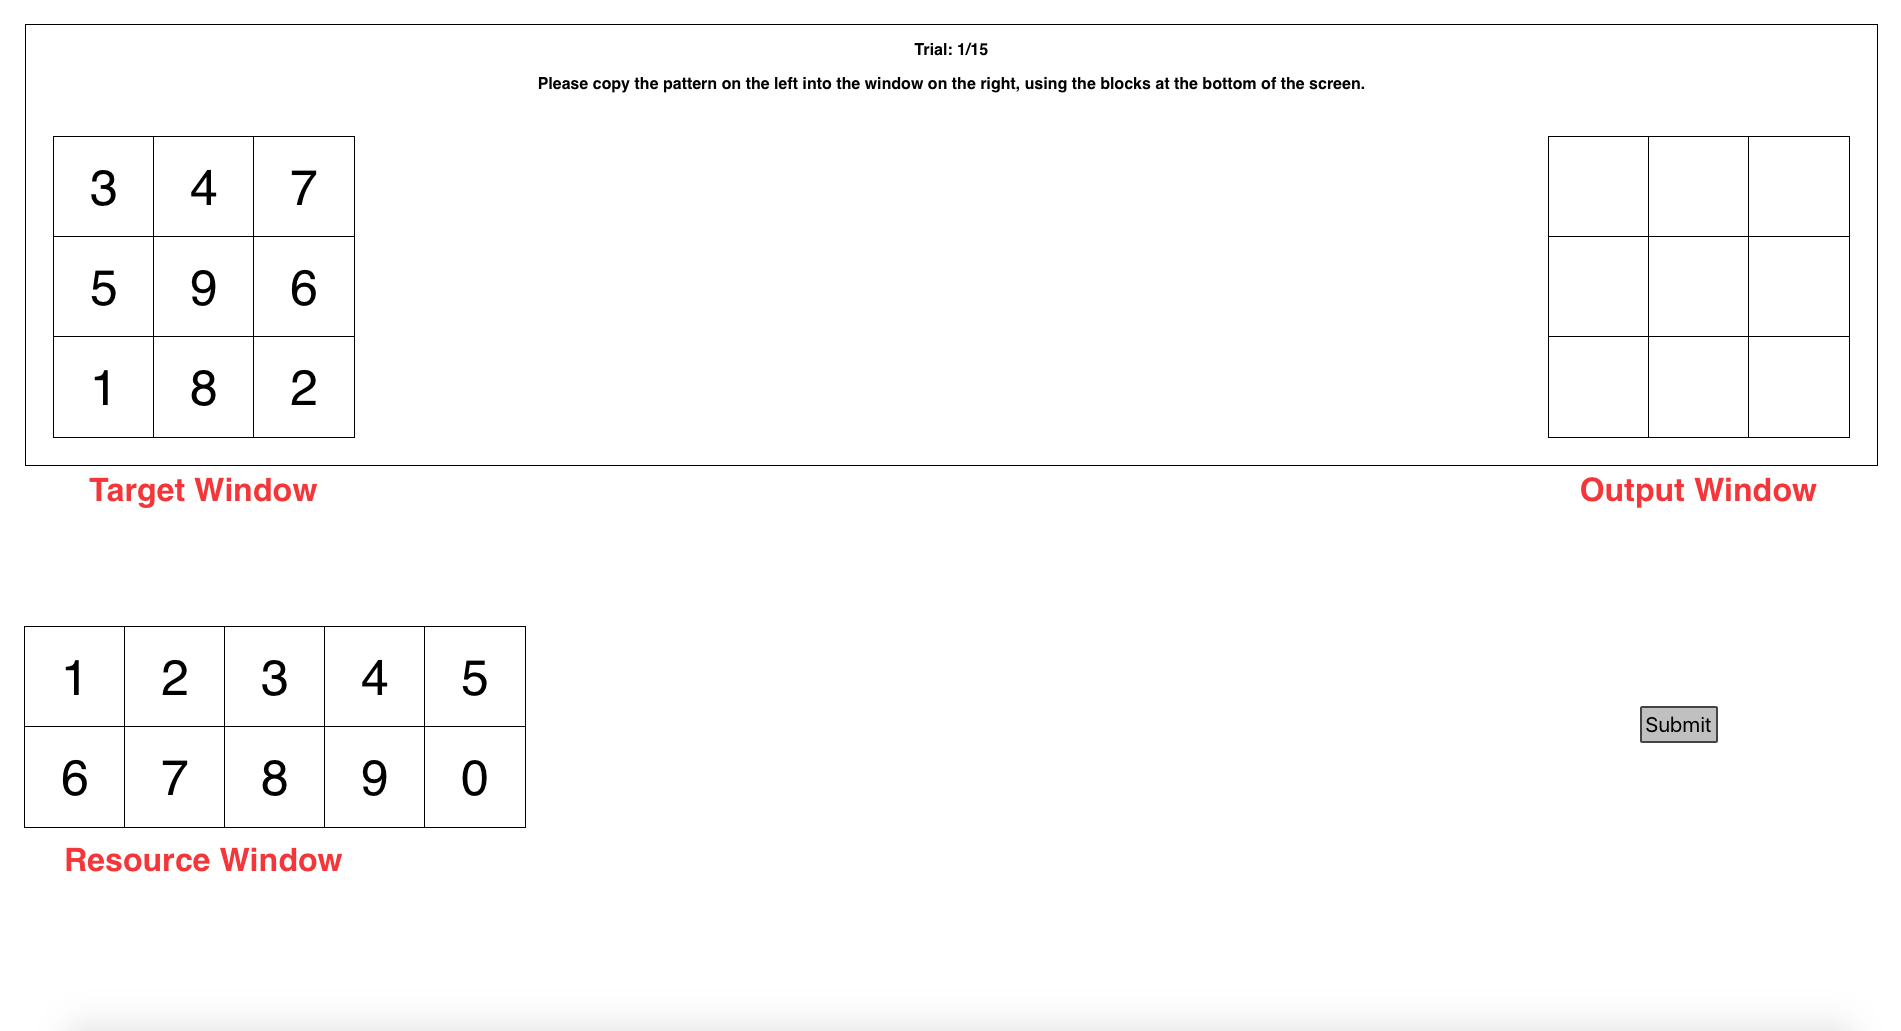
\includegraphics[scale=0.23]{images/ch34/ch4_numbers.png}}
\caption{The number condition.}
\label{fig:ch4_BWT}
\end{subfigure}
%\hfill%
\begin{subfigure}[b]{0.5\textwidth}
\centerline{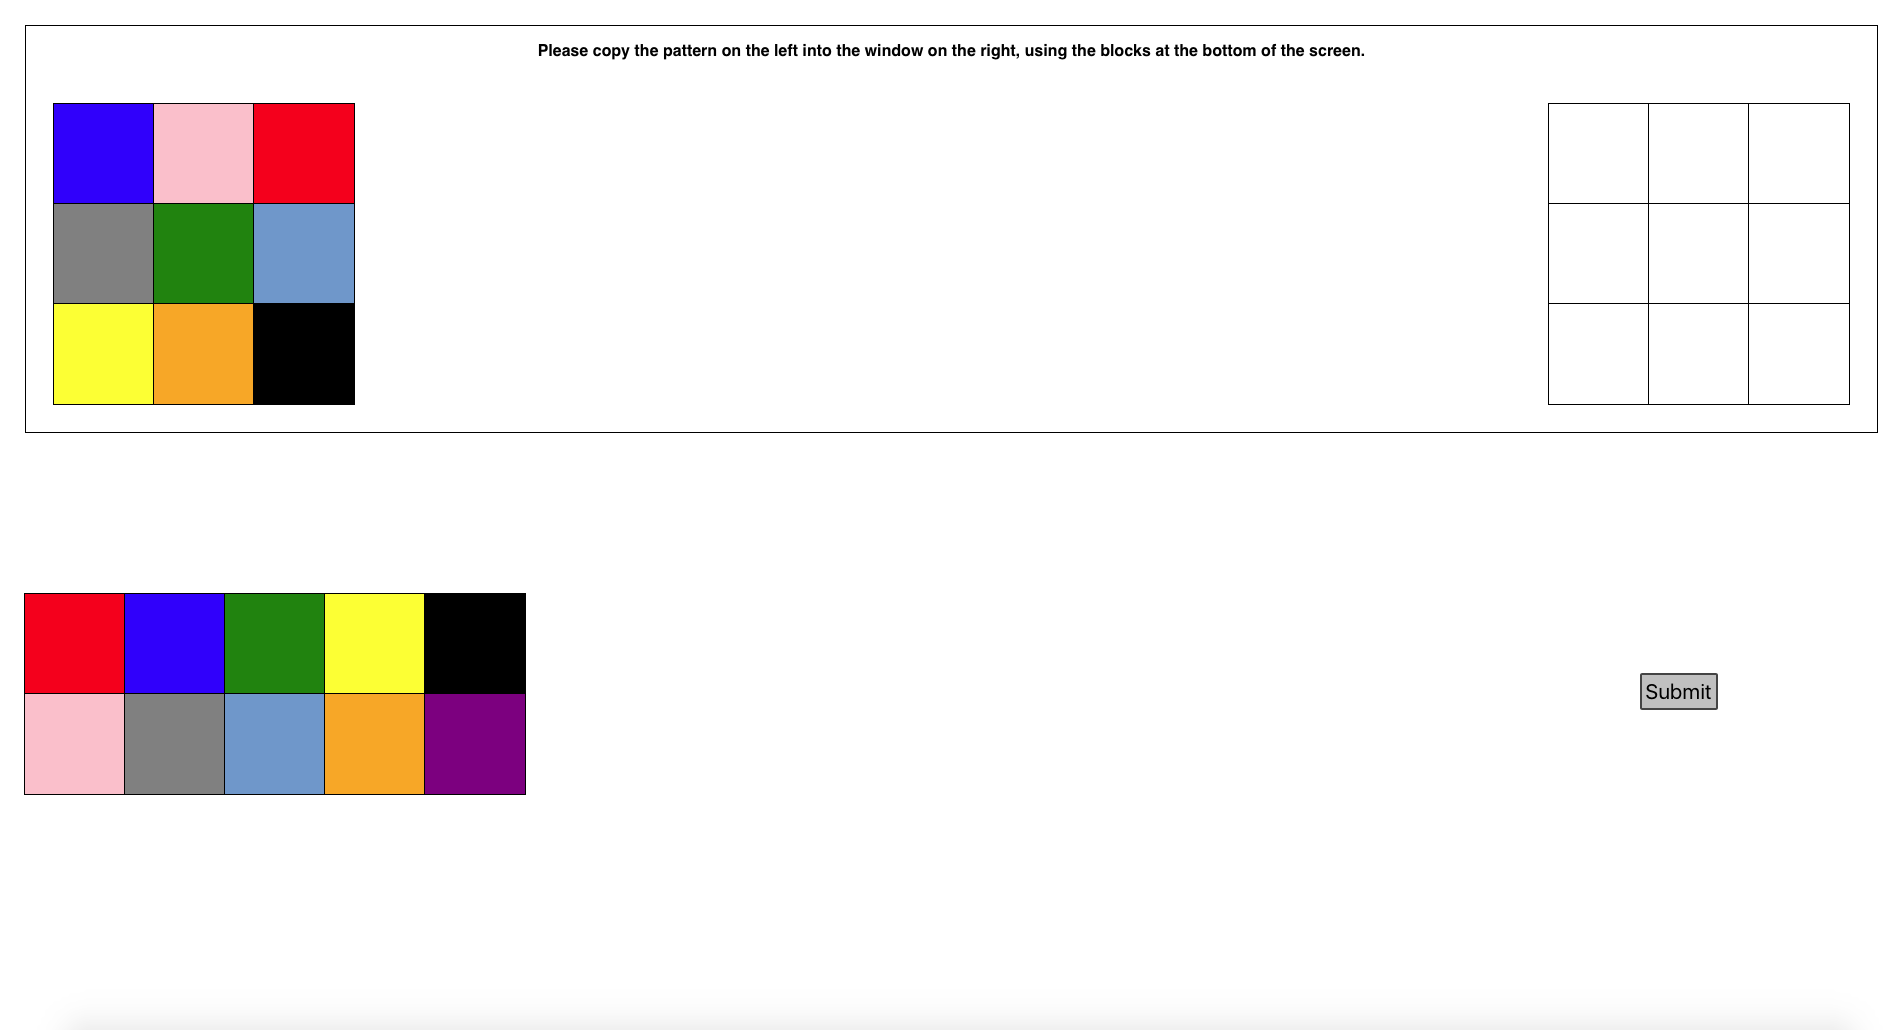
\includegraphics[scale=0.23]{images/ch34/ch4_colours.png}}
\caption{The colour condition.}
\label{fig:ch4_NWT}
\end{subfigure}
\caption[Study 3 task lay-out]{The task lay-out with the three different components.}
\label{fig:ch4_taskparadigm}
\end{center}
\end{figure}

Figure \ref{fig:ch4_taskparadigm} shows the task paradigm that was used. Each colour or number was only used once. The colours used were similar to the colours used in previous BWT studies \citep[e.g.][]{Gray2006, Morgan2009}.
Participants had to copy and complete fifteen patterns of each block type, and each participant had to copy over the same patterns. The target window showed a 3x3 grid with either coloured or numbered blocks. The output window showed an empty 3x3 grid, and was the same size as the target window. Participants had to copy the pattern shown in the target window by dragging blocks from the resource window and moving them into the output window. 

%Apparatus
The study was conducted on a desktop computer, using a 24-inch monitor with a resolution of 2048 x 1152 pixels. Participants used a computer mouse to drag and drop blocks. The experimental task was implemented using HTML, Javascript and PHP and run in a browser.  All relevant browser events, such as mouse movements to (un)cover the grey mask, dragging and dropping the blocks and mouse clicks, were recorded and saved in a mySQL database. The browser window covered the whole screen to minimise distractions.

For the Low IAC condition, eye fixations were used to measure the number and duration of visits to the target window. Eyetracking data was also obtained for the Medium and High IAC conditions. However, this data was not used due to the fact that people were able to also view the target window area whilst the target pattern was covered. Therefore, in accordance with previous IAC studies \citep[e.g.][]{Gray2004}, for the Medium and High IAC conditions the number and duration of uncovering the mask was taken as a measurement for visits to the target window.  These uncoverings were measured by Javascript. The usefulness and limitations of using these measures are discussed in the Discussion.

A Tobii T60 eyetracker was used for recording people's eye fixations. Eye movements were recorded at a rate of 60 gaze data points per second for each eye, with an accuracy of 0.5 degrees and timestamp accuracy of 4 ms. For the analysis, all consecutive eye fixations with no drag or drop actions in-between were added together and counted as one fixation.

\subsubsection{Procedure}
Participants were welcomed and briefed about the experiment. It was explained they would be shown nine blocks which were in a certain order, and had to copy this order by moving blocks around. Participants were instructed to complete the task as fast as possible, but it was explained that they were not able to continue until they had copied a pattern correctly. 
The experiment was broken down in two parts, one where they had to copy colours, and one where they had to copy numbers. For each part, they were given two practice trials first to get familiar with the set-up, and to give them a chance to ask questions if anything was unclear. There was an opportunity for the participant to take a break between the two parts. 
They were then asked to read and sign a consent form and given an information sheet with a summary of the study and the researcher's contact details. In addition to the verbal briefing, the explanation of the study was written out on the computer screen for the participant to read and they were shown an instruction video that showed how the experiment worked. The study took around 20-30 minutes to complete.

\subsubsection{Ethical considerations}\label{sec:quanethics}
The study was undertaken with ethical approval from the UCL Research Ethics Committee [Project ID Number UCLIC/1415/001/Staff Brumby/Borghouts]. 
At the start of each study, participants were first briefed verbally about the study. They were asked to read and sign a consent form, and were given an information sheet to keep. This information sheet contained a summary of the study information and the researchers' contact details. It was explained that an eyetracker would record their eye fixations and movements, but that these recordings were anonymous and that they would not be directly identifiable. After participants had completed the first part of the experiment, a prompt appeared on the screen advising them to take a short break. Participants could take a break as long as they wanted and could decide themselves when to continue with the second part of the experiment.

Participants were informed that the data would be used for research purposes only and stored in accordance with the Data Protection Act 1998. They were also informed that their data would be anonymised and when used in a report or academic paper, their data would not be directly identifiable. 
 
\subsection{Results}
The means and standard deviations of all dependent variables are shown in Table \ref{table:ch4_IACmeans}.

Eight participants were removed from the analysis due to weak eye-tracking calibration. Furthermore, one participant misunderstood the experiment and did not know she was allowed to uncover the mask of the target window more than once. This participant had scores that were more than three times the interquartile range from the rest of the participants' scores on six different variables, so this participant was considered an outlier and removed from the analysis. 

%\begin{table}
%\centering
%\ra{1.3}
%\begin{tabular}{|p{6cm}|lll|lll|}\toprule
\begin{tabular}{@{}p{6cm}lllclll@{}}\toprule %\begin{tabular}{  p{6cm} l p{1cm} l p{2cm} l  p{1cm}l p{1cm} | p{2cm} | p{1cm}|}
 & \multicolumn{3}{c}{\textbf{Colours}} & \multicolumn{3}{r}{\textbf{Numbers}} \\
 \cmidrule{2-4} \cmidrule{6-8}
 & Low & Medium & High && Low & Medium & High\\\midrule
\textbf{Strategy measures}\\
Number of visits to target window & \textbf{6.36} & \textbf{4.24} & \textbf{2.98} && \textbf{5.10} & \textbf{2.03} & \textbf{2.05} \\
						    & 		    2.28 & 		1.62   & 	          0.90 && 		2.48   & 	         0.63  & 	       0.67 \\
Visit time of first visit (s)  		    & \textbf{0.39} & \textbf{0.04} & \textbf{2.18} && \textbf{0.51} & \textbf{0.04} & \textbf{1.49} \\
				       		    &              0.23   & 		  0.02  & 	         1.59  && 		 0.45  & 	         0.05 & 	      1.01 \\
Average time of visits (s)  		    & \textbf{0.29} & \textbf{0.04} & \textbf{1.54} && \textbf{0.35} & \textbf{0.04} & \textbf{1.07} \\
				       		    &              0.13   & 		  0.02  & 	         0.95  && 		 0.15  & 	         0.03 & 	      0.77 \\
Number of blocks copied		    & \textbf{1.90} & \textbf{3.55} & \textbf{4.52} && \textbf{2.44} & \textbf{6.18} & \textbf{6.33} \\
 after first visit 		       		    &              1.84   & 		  1.93  & 	         1.43  && 		 1.89  & 	         1.61 & 	      1.67 \\
Number of blocks copied correctly & \textbf{1.86} & \textbf{3.22} & \textbf{4.07} && \textbf{2.36} & \textbf{5.96} & \textbf{5.98} \\
after first visit 		       		    &              1.75   & 		  1.83  & 	         1.20  && 		 1.74  & 	         1.52 & 	      1.55 \\

\vspace{10pt}

\textbf{Global task performance measures}\\
Number of incorrectly placed blocks 
				  		    & \textbf{0.15} & \textbf{0.67} & \textbf{0.79} && \textbf{0.17} & \textbf{0.31} & \textbf{0.46} \\
(per trial) 				       	    &              0.18   & 		  0.40  & 	         0.44  && 		 0.19  & 	         0.18 & 	      0.16 \\
Number of incorrectly submitted
				  		    & \textbf{0.27} & \textbf{1.9} & \textbf{2} && \textbf{0.36} & \textbf{0.5} & \textbf{0.83} \\
trials (per experiment block)	    &              0.65   & 		2.51 & 	   2.13  && 		 1.21  & 	         1.08 & 	      1.03 \\
Trial completion time incl. lockout
				  		    & \textbf{19.60} & \textbf{25.40} & \textbf{31.80} && \textbf{19.47} & \textbf{20.83} & \textbf{25.95} \\
(s)						    &                2.98   & 		5.16 & 	   	     6.08  && 	         3.03  & 	        3.08   & 	         4.21 \\
Trial completion time excl. lockout
				  		    & \textbf{19.60} & \textbf{25.40} & \textbf{28.84} && \textbf{19.47} & \textbf{20.83} & \textbf{23.89} \\
(s)						    &              2.98   & 		5.16 & 	   6.34  && 		 3.03  & 	         3.08 & 	      4.06 \\

\bottomrule
%\caption[Study 3 descriptive measures]{The effect of IAC on copying colours and numbers. The means are shown in bold, the standard deviations are below the means.}
\end{tabular}
\label{table:ch4_IACmeans}
%\end{table}

\subsubsection{Task strategies}

\subsubsection{Number of visits to the target window}
Participants made fewer visits to the target source when they had to copy numbers (M = 3.06, SD = 2.08) than when they had to copy colours (M = 4.49, SD = 2.18), F(1,30) = 41.62, p<.001, $\eta^2$  = 0.58. Participants also made fewer visits as IAC increased from Low (M = 5.73, SD = 2.41), to Med (M = 3.13, SD = 1.65), to High (M = 2.51, SD = 0.91), F(2,30) = 15.16, p<0.001, $\eta^2$  = 0.50. To investigate differences between conditions, post-hoc Tukey comparisons were performed. Results showed that participants made significantly fewer visits in the Medium-IAC condition than in the Low-IAC condition, p <.01. However, there was no difference in number of visits between the Medium-IAC and the High-IAC conditions, p=.59. Participants looked at the target window for colours more on every level of IAC (see Figure \ref{fig:ch4_noVisits}), and so there was no significant interaction, F(2,30) = 2.82, p=.08, $\eta^2$  = 0.16. 

\begin{figure}[!ht]
\centering
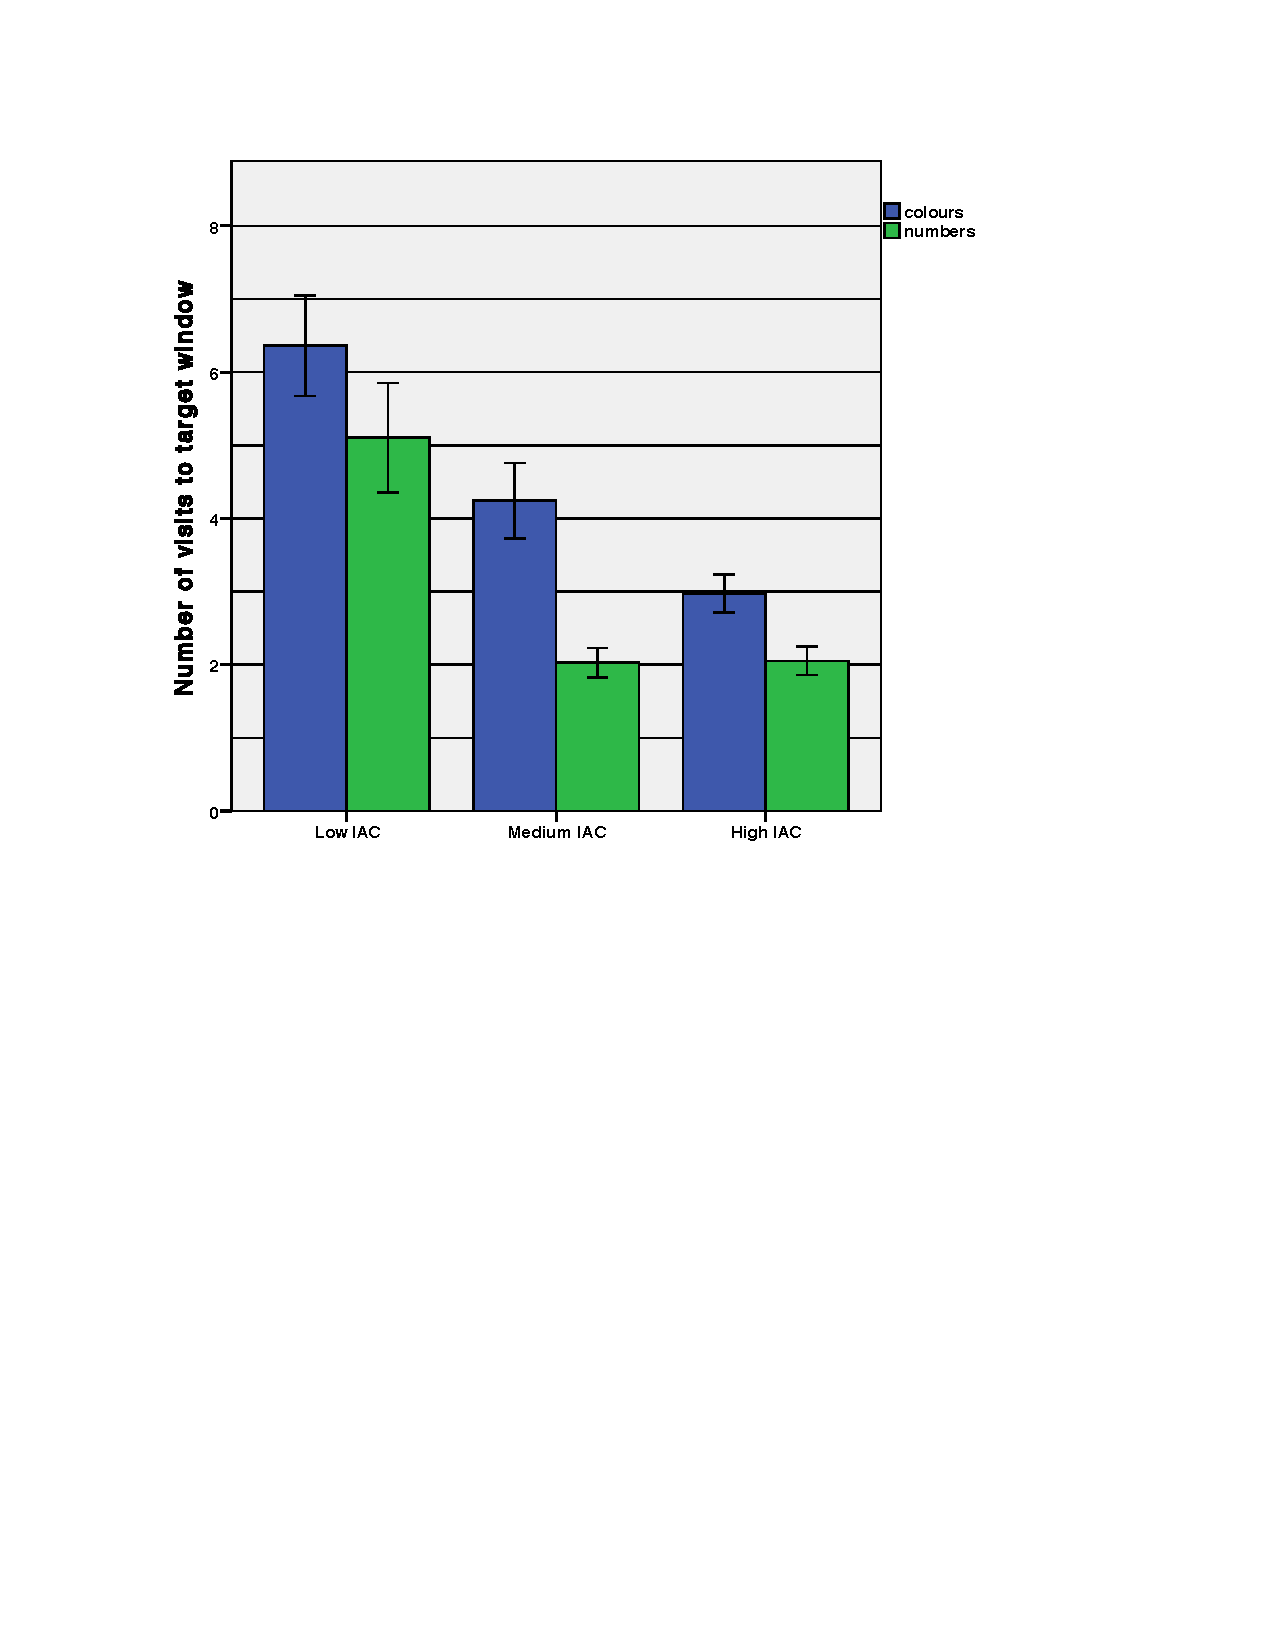
\includegraphics[width=\textwidth]{images/ch34/ch4_noVisits-bargraph.pdf}
\caption[Study 3 number of visits]{The interaction between block type and IAC for number of visits to the target window. The error bars represent $\pm $1 standard error.}
\vspace{-9pt}
\label{fig:ch4_noVisits}
\end{figure}

\subsubsection{Duration of first visit to target window}
There was no significant main effect of block type on the duration of the first visit, F(1,30) = 3.05, p=.09, $\eta^2$  = 0.09. Participants looked longer at the target source as IAC increased from Low to High. Post-hoc comparisons showed that participants looked longer in the High-IAC condition (M=1.84, SD = 1.35) than in the Low/Medium-IAC conditions, ps <.001. However, there was no difference in duration between the Low-IAC (M = 0.45, SD = 0.46) and the Medium-IAC (M = 0.05, SD = 0.04) conditions, p=.47. There was a significant interaction effect between IAC and block type, F(2,30) = 5.70, p<.01, $\eta^2$  = 0.28 (see Figure \ref{fig:ch4_firstVisitDuration}). There were no difference between block types in the Low-IAC condition, t(10) = -1.86, p = 0.09, nor the Medium-IAC condition, t(9) = -0.29, p = 0.7. However, in the High-IAC condition, participants looked significantly longer for colours (M = 2.18, SD = 1.59) than numbers (M = 1.49, SD = 1.01), t(11) = 2.76, p = 0.02.

\begin{figure}[!ht]
\centering
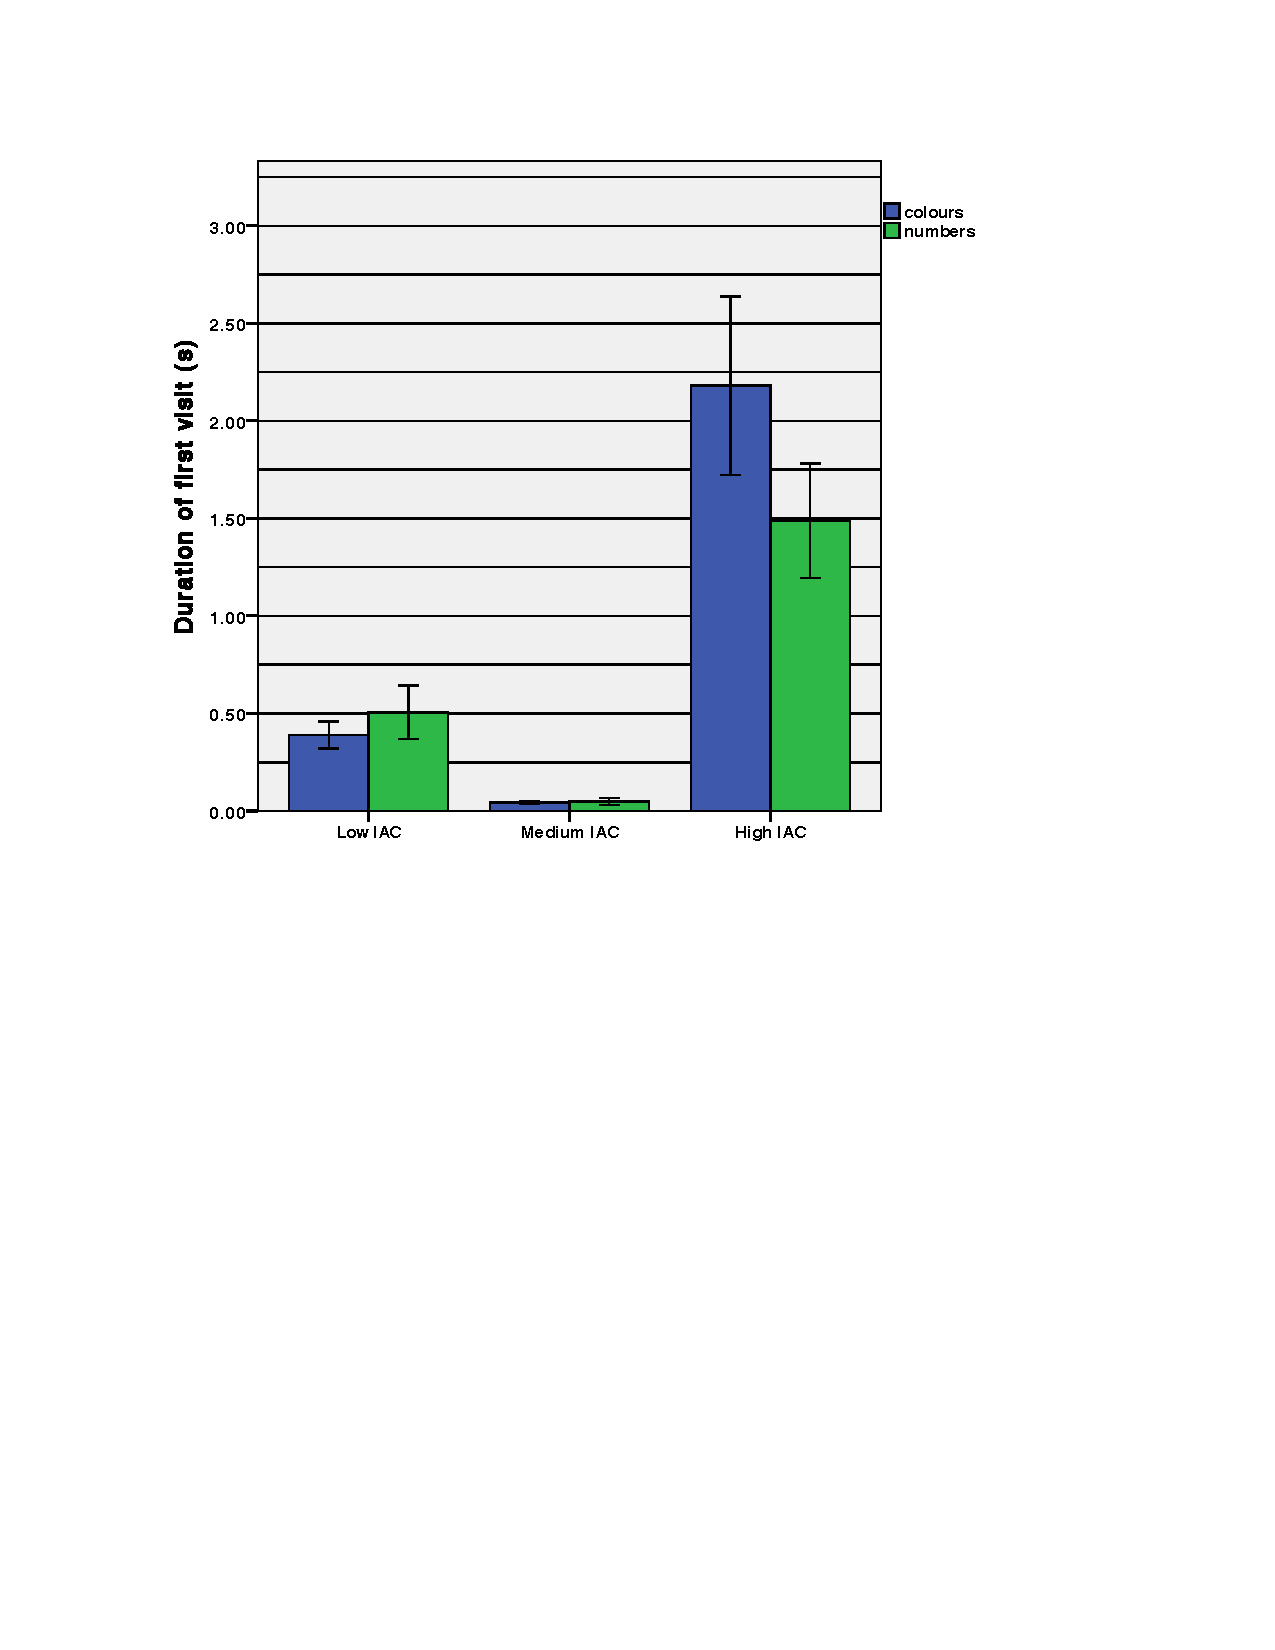
\includegraphics[width=\textwidth]{images/ch34/ch4_firstVisitDuration-bargraph.pdf}
\caption[Study 3 duration of first visit]{The effect of IAC on the duration of the first visit to the target window. The error bars represent $\pm $1 standard error.}
\vspace{-9pt}
\label{fig:ch4_firstVisitDuration}
\end{figure}

\subsubsection{Blocks placed after first visit}
People placed more blocks correctly after the first visit for numbers (M = 4.77, SD = 2.33) than colours (M = 3.08, SD = 1.81), F(1,30) = 63.86, p<.001, $\eta^2$  = 0.68. They also placed more blocks as IAC increased, F(2,30) = 12.54, p<0.001, $\eta^2$  = 0.46. Tukey post-hoc comparisons show there was a difference between the Low IAC and Medium/High IAC conditions (ps<.01), but not between Medium and High IAC conditions (p=.77). There was a significant interaction effect between IAC and block type, F(2,30) = 8.96, p<.01, $\eta^2$  = 0.37  (see Figure \ref{fig:ch4_firstCorrectBlocks}). When IAC was Low, the number of blocks that were copied correctly after the first visit did not differ significantly for colours or numbers.

\begin{figure}[!ht]
\centering
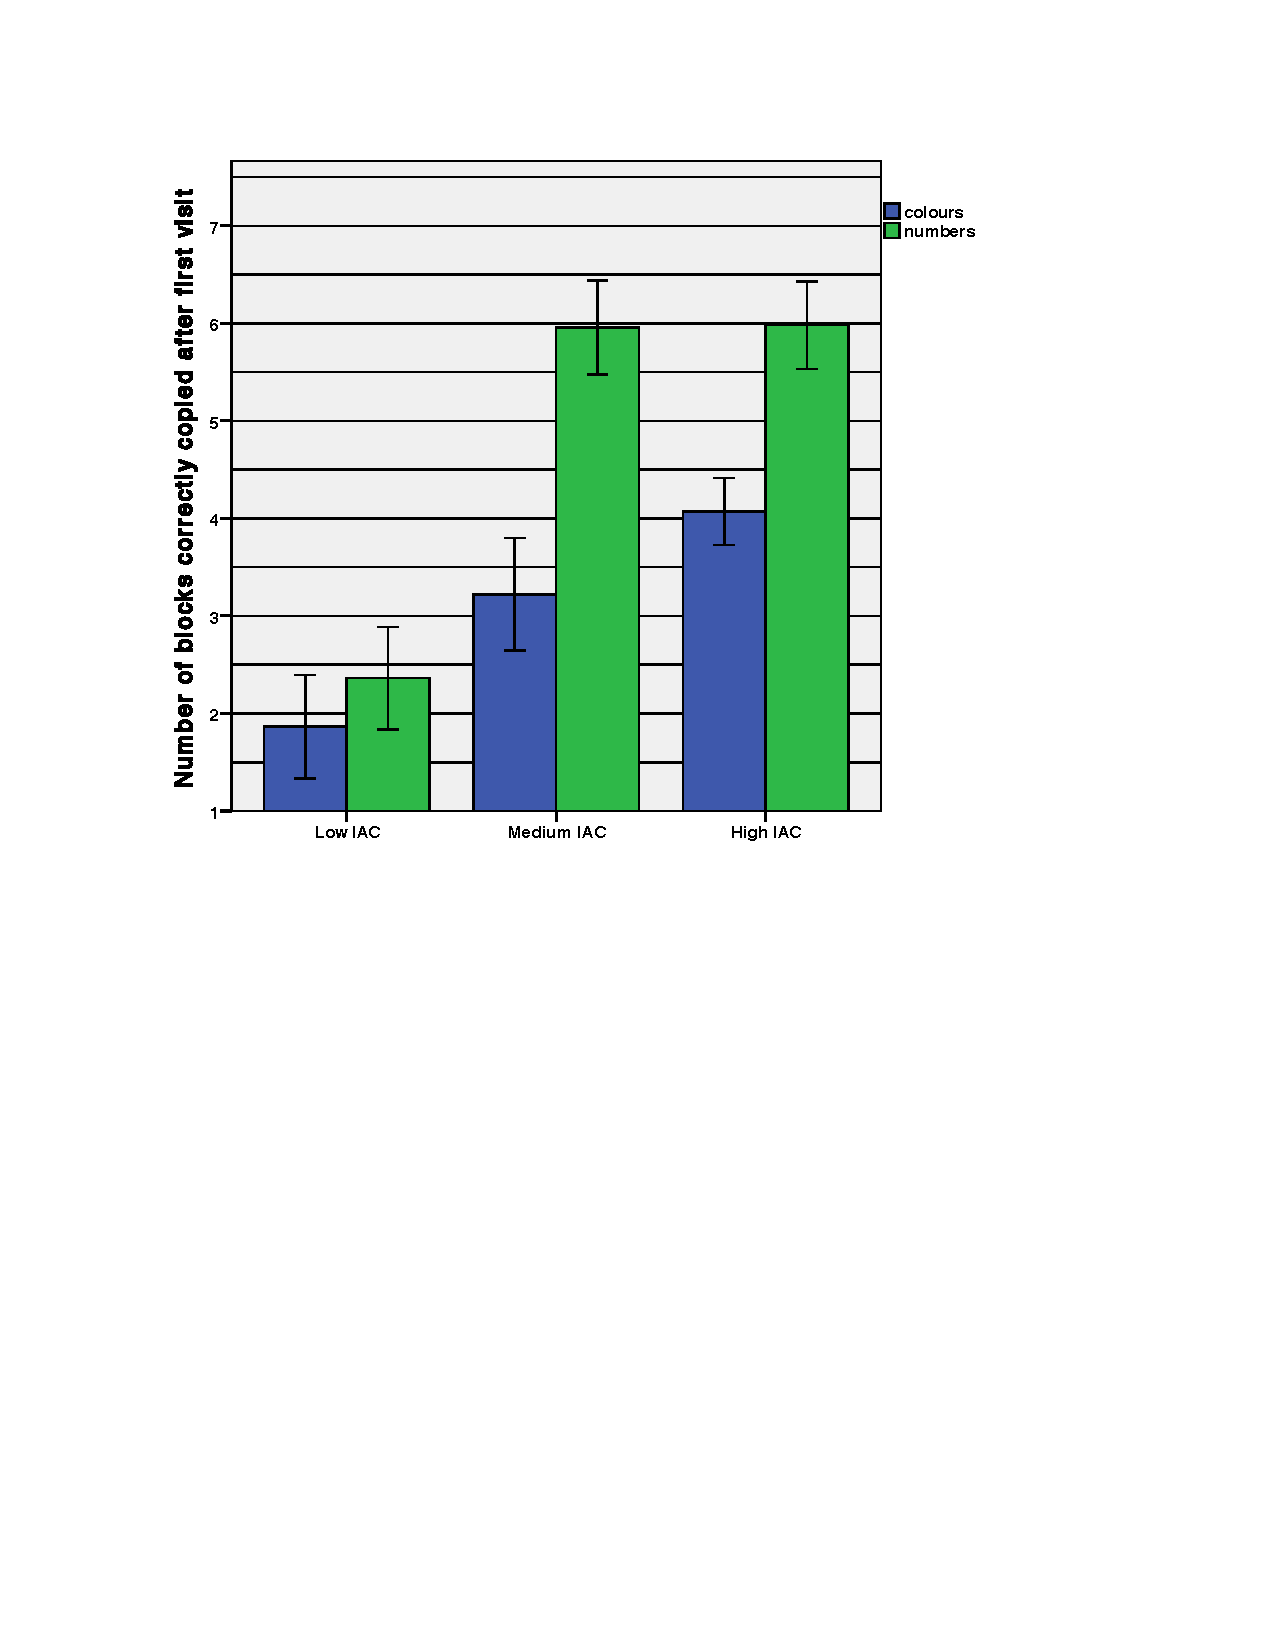
\includegraphics[width=\textwidth]{images/ch34/ch4_firstCorrectBlocks-bargraph.pdf}
\caption[Study 3 number of blocks correctly placed]{The interaction between block type and IAC for number of blocks correctly placed after the first visit to the target window. The error bars represent $\pm $1 standard error.}
\vspace{-9pt}
\label{fig:ch4_firstCorrectBlocks}
\end{figure}

\subsubsection{Global task performance}
The interactions between block type and IAC on global task performance measures all had the same trend: people performed the same for colours and numbers when IAC was Low, but differences appeared between the block types as IAC increased. As this trend was the same for each interaction, the statistical results of the interactions are reported but their specific trend will not be repeated.

\subsubsection{Number of incorrectly placed blocks}
Participants placed more blocks incorrectly for colours (M = 0.54, SD = 0.45) than numbers (M = 0.32, SD = 0.21), F(1,30) = 10.71, p=.003, $\eta^2$ = 0.26. As IAC increased and participants were keeping more items in memory, they increasingly placed more incorrect blocks, F(2,30) = 14.71, p<.001, $\eta^2$ = 0.50. Tukey post-hoc comparisons show there was a difference between the Low IAC condition (M = 0.16, SD = 0.18) and Medium/High IAC conditions (ps<.01), but not between the Medium (M = 0.49, SD = 0.35) and High IAC conditions (M = 0.63, SD = 0.36) (p = .3). There was a significant interaction effect between IAC and block type, F(2,30) = 3.36, p<.05, $\eta^2$ = 0.18. When IAC was Low, the number of blocks that were copied incorrectly did not differ significantly for colours or numbers, but as IAC increased, participants placed more blocks incorrectly for colours.

\subsubsection{Number of incorrectly submitted trials}
The number of trials that were submitted incorrectly was generally low, but participants submitted more incorrect trials for colours (M = 0.1, SD = 0.16) than numbers (M = 0.04, SD = 0.08), F(1,30) = 5.28, p=.029, $\eta^2$ = 0.15. There was no significant effect of IAC, F(2,30) = 2.70, p=0.08, $\eta^2$ = 0.15, nor any interaction, F(2,30) = 1.65, p=.2, $\eta^2$ = 0.10.

\subsubsection{Trial time}
Two trial completion times are considered here: total time and time excluding lockout. 
Looking at the actual completion time, participants took longer to complete a trial when they were copying colours (M = 25.80, SD = 7.06) compared to when copying numbers (M = 22.24, SD = 4.47), F(1,30) = 44.08, p<.001, $\eta^2$ = 0.60. As IAC increased from Low to Medium to High, participants took longer to complete a trial, IAC, F(2,30) = 15.91, p<0.001, $\eta^2$ = 0.52. Tukey post-hoc comparisons show there was a difference between Low/Medium and High (ps<.01), but not between Low and Medium (p = .12). There was a significant interaction effect between IAC and block type, F(2,30) = 11.05, p<.001, $\eta^2$ = 0.42. 

With the lockout time in the High-IAC condition removed, the same effects were found for block type, F(1,30) = 34.55, p<.001, $\eta^2$ = 0.54, and IAC, F(2,30) = 8.18, p=0.001, $\eta^2$ = 0.35. Tukey post-hoc comparisons show there was still a difference between Low and High (p=.001), but no longer between the Medium IAC and Low IAC or High IAC conditions (ps >.1). There was a significant interaction effect between IAC and block type, F(2,30) = 8.13, p=.002, $\eta^2$ = 0.35.

\subsubsection{Qualitative data}
The screen recordings from the eye-tracker were played back to further investigate people's behaviour. Although this helped understand some behaviour which could not be determined from the quantitative data alone, these observations only serve to explain some of the quantitative measures and are not the main focus of the analysis.

The visit durations in the Medium IAC condition were suspiciously short. Upon replaying the screen recordings, it appeared that participants often accidentally moved their cursor over the grey mask of the target source. This was counted as a visit by the program, even though participants may have not intentionally moved their cursor to this part of the screen to look at the target source. They did not spend a long time looking at the target window, but also did not immediately move blocks either, and sometimes waited multiple seconds before they made a move. 

\begin{figure}[!ht]
\centering
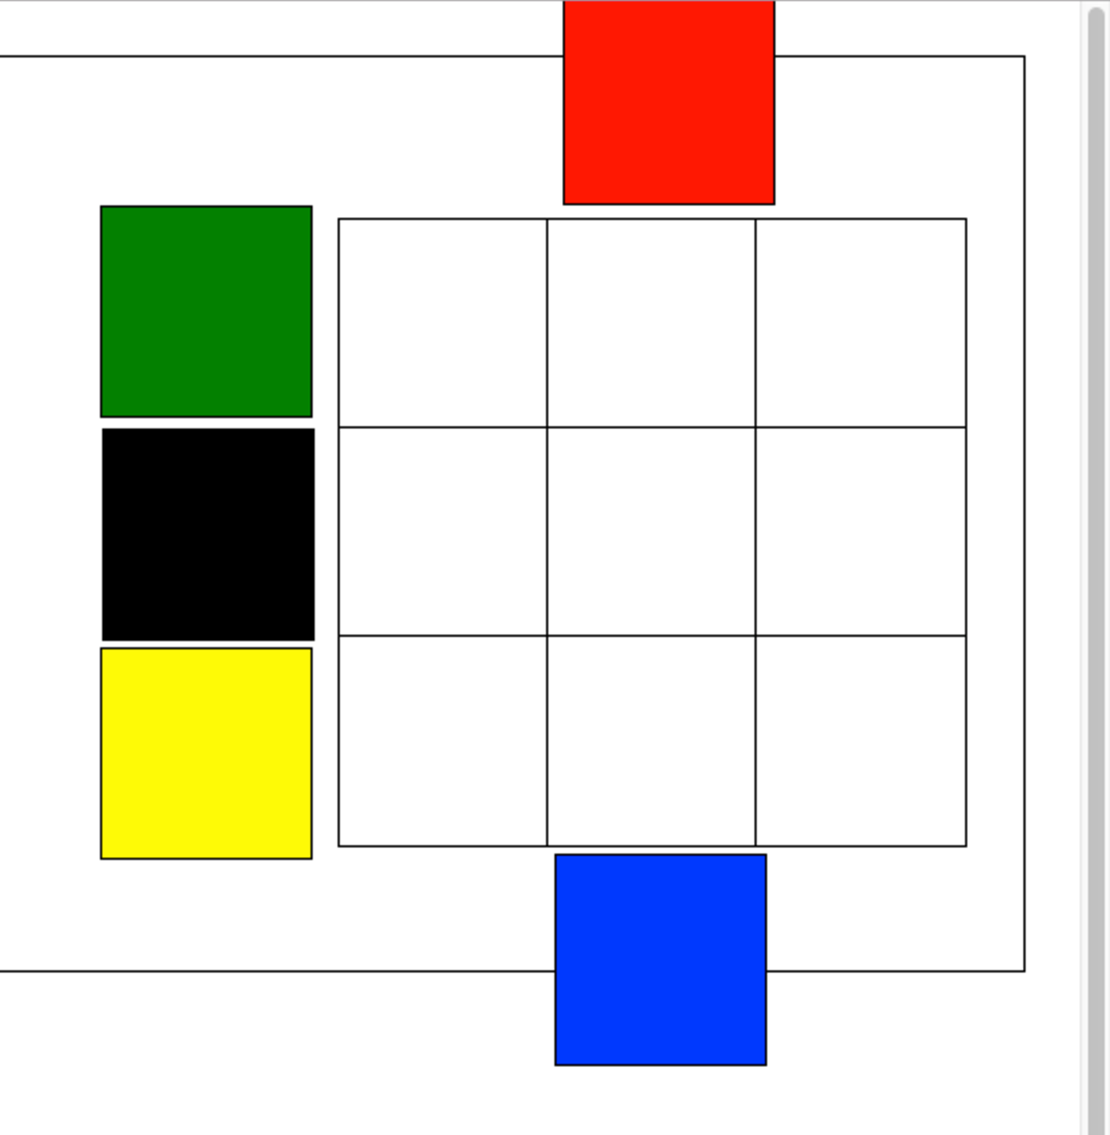
\includegraphics[scale=0.3]{images/ch34/ch4_placeholders.pdf}
\caption[Study 3 placeholders]{Participants placed blocks outside of the output window as `placeholders'.}
\vspace{-9pt}
\label{fig:ch4_placeholders}
\end{figure}

During the 1-s lockout in the High IAC condition, participants changed their minds about visiting the target window on numerous occasions. They placed their mouse cursor on the mask, but left this field before it was uncovered to move one or more blocks. It could be this decision also occurred in the Medium IAC condition, but as there was no lockout the mask was already uncovered before people made this decision, and would explain the very short visits.

People sometimes placed the blocks as `placeholders' as shown in Figure \ref{fig:ch4_placeholders}: they placed several blocks outside of the output window next to the position they thought it belonged to, but did not place it there yet. Only after viewing the target again, they placed the blocks in the output window. Looking at quantitative data alone, this type of strategy would be depicted as one long view at the target, after which all blocks were placed in one go. This is true to some extent, but as people could already place the blocks and offload their memory without this being recorded by the program, they only had to check if this position was correct on the subsequent visit, and is different from a strategy where people spent a long time trying to memorise the blocks after which all blocks were placed.


\newpage

\subsection{Discussion}
This study replicated the Blocks World Task with the aim to see if the effect on IAC on a copying task, as previously found when using colours, can be extended to copying numbers, and if a deeper encoding of numbers into memory makes people more accurate.

The main findings are:

\begin{itemize}
\item
Numbers are easier to copy than colours, but only if IAC is increased
\item
Increases in IAC make people adopt memory-intensive strategies
\item
Increases in IAC increases errors
\end{itemize}

\subsubsection{The effect of block type on task strategies and performance}
Changing the block type from colours to numbers made it easier to memorise the blocks: people made shorter and fewer visits than when copying colours, but were still able to place more blocks. This difference in performance is only found in the Medium and High IAC conditions, which further suggests the difference between numbers and colours is due to the memorability of the information, and the interactions on most of the dependent variables further show that the difference between block types was dependent on the level of IAC.

The difference between numbers and colours fit well with the distinction in Baddeley's \citeyearpar{Baddeley1986} seminal model of working memory between processing visuo-spatial and verbal information. As numbers can be rehearsed and therefore refreshed in working memory, they are likely easier to memorise. After the study had ended, several participants in this study explained they used some sort of rehearsal and tried to say the numbers out loud in their head. For colours, some indicated they tried to either capture a mental picture of the colours in their mind, while others rehearsed the word for each colour (e.g. 'red' and 'blue') but they felt they were able to remember fewer items using this strategy. This is consistent with \citet{Chincotta1999}'s finding that people have a greater memory span for Arabic numerals (e.g. 1, 2, 3) than corresponding words (e.g. one, two, three).

Though an increase in IAC made people rely on memory and people seemed to memorise numbers more easily than colours, an increase in IAC did not make people more accurate in copying numbers as in \citet{Gray2004}, where people had to memorise VCR programming information. The error rate for numbers was however already quite low in all conditions, and moreover people were not explicitly instructed or trained to memorise the information before each trial as in \citet{Gray2004}.

\subsubsection{The effect of IAC on task strategies and performance}
The effect of IAC on people's cognitive strategies, as found in previous studies, is replicated in this study: as the cost of accessing the target window increased, people increasingly relied on memory \citep{Gray2006, Morgan2009, Waldron2007}. People switched from a perceptual to a memory-based strategy by making fewer but longer visits to the target window and placing more blocks immediately after the first visit. This strategy worsened their global performance as they took longer to complete the task and placed more incorrect blocks throughout the trials. 

An increase in IAC also made people rely more on memory when copying numbers. When a mask was added over the target window, people visited the target window less often and they placed more blocks after the first visit. In both the Medium IAC and High IAC conditions, people on average placed around six blocks correctly after the first visit, after which they needed one more visit to look at the last three blocks. The average number of items people can memorise is 7$\pm$2 items \citep{Miller1956}, and potentially six blocks was the maximum that people could reasonably memorise.

In previous studies, adopting a memory-based strategy when copying text and numbers improved accuracy \citep{Gray2004, Soboczenski2013}. In the current study, the hypothesis that memorising numbers due to an increased IAC would make people more accurate is not supported. 
The error rate was overall low and upon reflection the interaction of moving blocks may have made people sufficiently slow to hardly make any errors. In \citet{Gray2004} and \citet{Soboczenski2013}, people typed in data using a computer keyboard.

With the BWT, it was difficult to measure visits to the target window in the same manner for all conditions. For the Low IAC conditions, eye fixations were used, whereas for the Medium and High IAC conditions, uncoverings of the mask were used. This introduced several problems. First, while eye-tracking measures show how long and how often people are looking at a particular part of the screen, it can not reveal if people are actually perceiving or processing the data that is displayed \citep{Waldron2007}. For the Medium and High IAC conditions, an interaction was required and a conscious decision had to be made to reveal the target in these conditions. It would therefore seem likely that uncoverings more reliably measure visits to the target window. However, the uncoverings for the Medium IAC conditions were suspiciously short. Playing back the screen recordings suggests participants often accidentally uncovered the window, and it is therefore less clear if these are a reliable measure of actual visits. 

\subsubsection{Summary}
The purpose of this study was to study the effect of IAC on strategy, speed and accuracy when copying from one source, and investigate if the effect of IAC, as found in previous experimental studies, would extend to copying numbers. In order to be able to compare results of this study with previous IAC studies the same task paradigm of the Blocks World Task was used.

The hypothesis that people would need fewer switches and would perform better for numbers than colours is supported, indicating that numbers are easier to memorise. The hypothesis that memorising numbers due to an increased IAC would make people perform better is not supported. The error rate was overall low and upon reflection the interaction of moving blocks may have made people sufficiently slow to hardly make any errors. Furthermore, in Study 1 people saved up data to enter a lot in one sequence, and errors increase as people have to copy more \citep{Healy2004}. Potentially the setup of this experiment was not suitable to reliably measure an increase in errors.
 
The information was copied from one source, and for each participant the IAC was the same throughout the experiment: it was either low, medium, or high. Therefore, while using the BWT task paradigm was appropriate in comparing its results with previous IAC studies, it did not resemble the data entry tasks observed in the financial office setting of Study 1. 

Considering these limitations, it was decided after this study to not continue with the same task paradigm, but certain learning points can be taken away from this study.  

First, the entry method matters. An entry method that is sufficiently slow may make people accurate, regardless of the level of IAC. 
Second, the effect of IAC generalises, but it is not clear how the results of this experimental paradigm can be translated in suggestions in how people dealing with differing levels of IAC can best be supported in their work. In contrast to this study, where information came from one source, and always had the same level of IAC for each participant, Study 1 showed that for entering expenses, people have to enter different types of information, these do not all come from the same source, and each source can have a different access cost.

Third, the measured short visits in the Medium IAC conditions may have confounded the results. In future studies, the setup of the experiment should be designed so that participants do not accidentally access the source when they do not intend to.

Lastly, for each dependent variable, the same consistent measure should be used to compare across conditions. This could be data provided by an eyetracker, or interaction measures such as mouse clicks, key presses or interkey intervals. 

The next study will try to more closely simulate the expenses task observed in the financial office setting of Study 1 and 2. People will have to enter and collect information from multiple sources with different IACs. The aim is to see how these differences in IAC influence people's switching strategies between entering and looking up data when copying from multiple sources. 

%In order to be able to further conduct experiments that study how people can best be supported when retrieving information for a data entry task, it is important to understand where they have to get it from. Therefore, the next study I will focus on the expenses task identified in Study 1 and look at the resources people need for this task, where they need to get it from, and how costly it is to access this information.


\section{Study 4: Copying data from multiple sources}
 
\subsection{Introduction}
Study 3 showed that as it takes longer to access an information source needed for a copying task, people spend a longer time looking at that source. They try to group and memorise as much information, in order to minimise the number of revisits to this source. Though people copied over more items after one visit using this strategy, they also made more errors overall. In the experiment, all information was to be found on a single source. People may have tried to memorise too much items in one visit, and upon entry relied on incorrectly memorised information in the head.

Data entry in office workplaces often does not involve a single source, but information can be spread over various sources. These sources are often not all equally easy or hard to access. How do people prioritise how they enter and look up information from these different sources? Do they enter the easy items first? And will they still try to group and memorise as many items? Or will they look up and enter items from one source at a time? In order to support people in looking up information for data entry work, it is important to first understand how people currently manage these information tasks.
% Study 1 and 2 showed that for an expenses task, people have to collect the data to enter from multiple sources. Some of these sources are easy to access such as paper sheets on a desk, while others have a higher IAC, such as a computer document or window that takes time to open and view.

In the contextual inquiry of Study 2, participants started data entry by first collecting all physical sources first and placing these on their desk. They then entered this information, which was nearby, first. They postponed accessing other sources until they needed to enter it during the task. If information took too long to access, they would set aside the task and continue with other tasks. One of the factors that influenced the different strategies appeared to be the time cost to retrieve the information. 

This study tests the assumption that observed strategies from Study 2 are influenced by the time costs to access information sources. Whilst prior studies have demonstrated that various tasks can involve the use of multiple information sources \citep{Cangiano2009, Murphy2016, Su2013}, there are limited studies that measure how people use these sources, and to what extent the time cost to access a source influences these decisions.

%Study 3 has given an understanding of the effect of IAC on people's switching strategies when copying from one information source. As IAC increases, people make fewer visits to the source and instead enter what is in their head. The current study aims to investigate how differences in IAC affect people's strategies in switching between entering and looking up information from multiple sources, and whether different strategies affect performance.

%The office setting of Study 1 and 2 will be simulated in a laboratory environment. Participants will have to retrieve data from a number of sources, and enter this into a desktop computer using keyboard and mouse. The sources will be made to resemble the sources identified in Study 1 and 2 and will be on paper, on a second computer screen, or on the same screen as where the participant has to enter the data. The data participants have to enter will be similar to data that is entered for an expenses task: this includes names, financial numbers, and alphanumeric strings. 

%Study 3 used eyetracking data and mouse movements to measure number and duration of visits to the target source. For the setup in this experiment, these measurements are not possible for visits to paper sources with the eyetracking equipment available. I will therefore video record and/or observe participants and code the timing and number of visits people make to the different information sources. To supplement these with quantitative measures, I will also measure keylogging data to get further insight whether and how long people interrupt entering data, presumably to retrieve data. In accordance with \citet{Gould2016}, intervals of more than 5s are considered to be an interruption. 

%A within-subjects design will be used. The independent variables will be type of data (e.g. names, financial numbers, and alphanumeric strings), and IAC of the information sources. Dependent variables will be number of visits to sources, timing of visits, resumption lag, interkey intervals, typing speed, and error rate.

%The identified behaviour of how people manage looking up information is used to create a set of design recommendations for the current expenses system, which are evaluated in the next chapter.

The following questions will be addressed:
%\begin{itemize}
%\item[RQ1.] \textit{How does IAC affect the number of visits to look up information from multiple sources with different IACs?}
%\item[RQ2.] \textit{How does IAC affect the order of visits to look up information from multiple sources with different IACs?}
%\item[RQ3.] \textit{Do the number and order of visits affect data entry accuracy and speed?}
%\end{itemize]

The soft constraints hypothesis predicts that people choose and adapt their task strategies in order to minimise time \citep{Gray2006}. Study 3 found that the longer it takes to access information, the more items people try to memorise in one visit. Based on these findings, the following hypothesis is made: 
\begin{itemize}
\item[H1.]
As IAC increases, people will try to group and memorise multiple items to minimise visits.
\end{itemize}

In \citet{OHara1998}'s study on the effect of IAC on problem solving tasks, participants in Low-IAC and High-IAC conditions initially performed the same type of strategies. However, over time participants in a High-IAC condition  learnt more efficient strategies, whilst participants in a Low-IAC condition continued to use the same strategy. Prior work has also shown that people who are exposed to High-IAC situations will continue to use the strategy they learnt to be the most efficient, even in situations where the cost to access information is no longer high \citep{Patrick2014}. It is therefore expected that once participants learn it is more efficient to group High-IAC items, they may adopt this strategy for Low-IAC items as well. In Study 2 of this thesis, people tried to enter items that were nearby in the environment first, and postponed looking up other information until later. Based on these findings, the following hypothesis is made: 
\begin{itemize}
\item [H2.]
As the experiment progresses and people become aware how costly it is to access certain sources, they will learn and choose to enter all the Low-IAC items first, in a batch, and then the High-IAC items second, also in a batch, rather than looking up each item as they need it. 
\end{itemize}

Lastly, if people group items and spend a longer time looking up information, this means they will be interrupted from their data entry task for a longer time. The longer people are interrupted from a primary task, the slower they are to resume that task after the interruption \citep{Monk2008}, and the more likely they are to make resumption errors  \citep[e.g.][]{Brumby2013}. Based on this, the following hypothesis is made:
\begin{itemize}
\item[H3.]
As IAC increases, people will be slower and make more errors.
\end{itemize}

\subsection{Method}
\subsubsection{Participants}
Thirty-three participants (12 male) ranging from 18-52 years (M = 26, SD= 8) took part in the experiment. They were recruited from a university subject pool and received $\pounds$4 for their participation.

\subsubsection{Task}
The experimental data entry task was framed around the expenses task from Studies 1 and 2. For this task, the user has to complete a number of data entries regarding incurred expenses in order to get the expenses reimbursed. They enter this into a claim form, which looks similar to a spreadsheet. Users can choose to either fill in multiple expenses in one sheet, in which each row corresponds to one expense, or have separate spreadsheets for each expense. The current experiment will use the scenario where users enter multiple expenses in one sheet.

For each trial, participants were presented with a data entry sheet consisting of two expense claims (see Figure \ref{fig:ch34_4-tasklayout}). They had to complete each row by entering a financial amount to specify an expense that was made, and an account code to specify which account the expense belonged to. The retrieved these data items by switching to two other pages. One page contained the amounts, and another page contained the account codes. The participant could go to a page by clicking on the corresponding name in the horizontal menu at the top of the screen. Only one page could be viewed at a time and covered the full screen. 

%The names of computer windows with an increased IAC were underlined, to make it easier to see which windows had an increased time cost to open.
\begin{figure}
 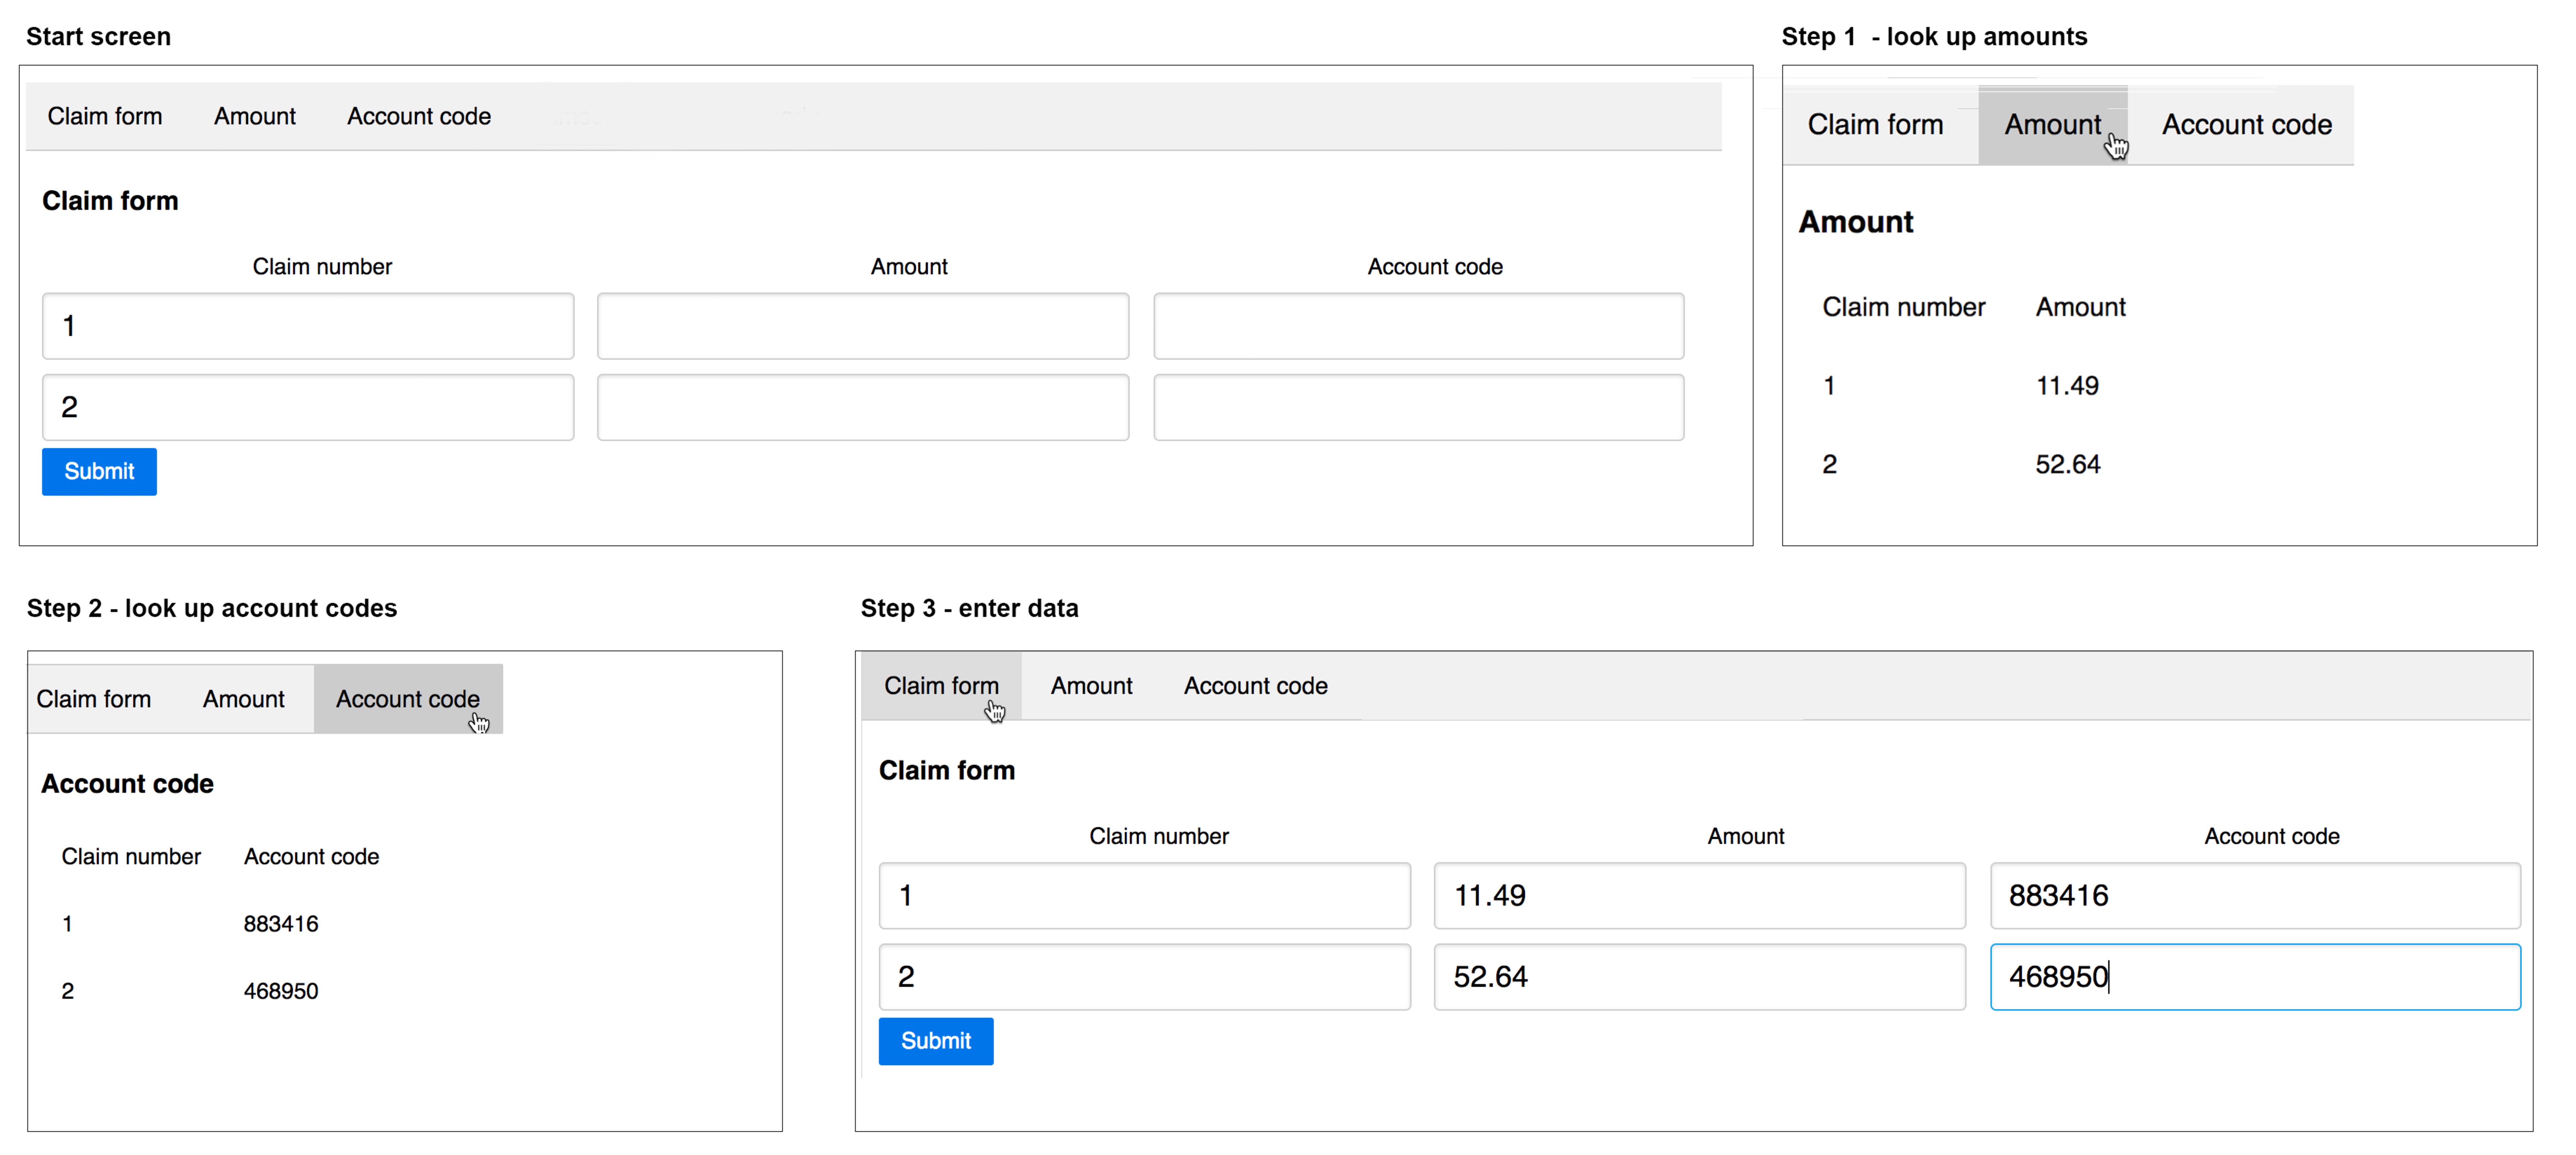
\includegraphics[width=\textwidth]{images/ch34/ch34-4_Tasksequence.pdf}
    \caption{The data entry task. At the start of each trial, participants were presented with a data entry form with two expense claims, and had to enter four data items in a data entry form. The data items were retrieved from a separate Amounts page (Step 1) and an Accounts page (Step 2) and entered into the data entry form (Step 3).}\label{fig:ch34_4-tasklayout}
\end{figure}

\subsubsection{Materials}
The numbers to be entered were made to resemble values that are ecologically relevant to the task. The account codes were similar to codes that are currently used by one of the universities studied in Chapter 3, and have a fixed length of six digits (e.g. 654273). Office workers at this university usually worked with the same 20 or 30 account codes. They were aware they worked with the same set of codes, but still had to look a code up each time they needed to enter it, as the codes were too difficult to enter from memory. The codes had a length of six digits, and the string was random with no pattern. Amounts consisted of two digits on the integer part and two digits on the fraction part (e.g. 11.95). 

%An experimental session consisted of 50 trials, divided into 5 blocks of 10 trials.  Each trial consisted of four data entries, so in total a participant made 200 entries. For each block, a set of 20 different amounts and 20 different account codes were used. These sets were re-used for every block, so in total, each number was presented five times throughout a session. There were two practice trials before the experiment began. The numbers used in the practice trials were not used for the experimental trials. The data items always had the same length: the amounts consisted of two digits on the integer part and two digits on the fraction part (e.g. 11.94), and the account codes were six digits (e.g. 654273).

The experiment was conducted in a maximised web browser on a desktop computer with a 24-inch monitor and a resolution of 2048x1152 pixels. Participants used a computer mouse and number keypad, and the option to copy and paste information was disabled. If the participant switched from the data entry form to another page and back, the cursor stayed in the same data entry field. The task interface was developed in HTML, CSS, JavaScript and PHP. All mouse clicks, key presses and timestamps were recorded using JavaScript.

\subsubsection{Design}
A between-participants design was used with one independent variable, the presence or absence of a delay when switching to one of the information pages. In the Control condition, there were no delays in switching between any of the pages. In the High-Amount condition, there was a 2-s delay when switching to the Amount page, and in the High-Account condition there was a 2-s delay when switching to the Account page. There were no delays in switching back to the data entry form. On a trial-by-trial basis, the main dependent variable was whether people interleaved or not: did participants enter the data items in sequential order, or did they interleave between the two expenses? Two values had to be entered for each expense: an amount and an account code. If participants entered the amount and account code of one expense before entering the other expense, this was considered a sequential order. If participants entered amounts of each expense first, followed by entering the account codes or vice versa, this was considered interleaving. All key presses were recorded to determine in which order data was entered. Page switches were recorded to capture the number and duration of switches to information pages. Other dependent variables were trial completion time and data entry error rate. In addition, we analysed the type of errors made to determine whether participants made more omission errors in any of the conditions. 

\subsubsection{Procedure}
The experiment took place in a closed quiet room. It was explained to participants that the task involved entering expenses, and that for each trial they had to enter two expenses. They were not advised to use a particular strategy, but it was explained it was important to complete all data entry fields before proceeding to the next trial, as they could not return as soon as they had pressed 'Submit'. There were no restrictions in the number or duration of times they could switch between pages, or the order in which they completed the trial. One trial consisted of two expenses, i.e. four data entries. Participants first completed two practice trials to familiarise themselves with the task, and were free to ask any questions; data from these trials were not included in the analysis. After that, the experimental session consisted of 50 trials, divided into 5 blocks of 10 trials. After each block, there was an opportunity for the participant to take a short break. A prompt appeared on the computer screen, and the recording time was paused. Participants could carry on with the experiment by pressing a button on the screen. For each block, a set of 20 different amounts and 20 different account codes were used. These sets were re-used for every block, so in total, each number was presented five times throughout a session. The experiment took approximately 30 minutes.

\subsubsection{Pilot study}
Two pilot studies were conducted with colleagues of the researcher to test the experimental design. In particular, the pilot studies aimed to see if the length of the experiment was long enough for participants to learn and develop  strategies, but not too long to tire the participant.

During the pilot studies, there was a scheduled break after every 5 trials. Both participants mentioned the break prompts happened too frequently, and experienced them as disruptive. They did not find the experiment too long. One participant could not remember which computer tabs had an increased IAC. As a result, he did not adapt his strategies according to anticipated IACs and entered the data items row by row. The second participant mentioned that the increased IACs definitely made her more careful in checking the numbers were correct. The participants were aware some of the numbers occurred more than once, but the numbers did not occur often enough to be able to memorise them. 

For the real experiments, the breaks were reduced to happen after every 10 trials. In addition, the names of information pages with an increased IAC were underlined in the horizontal menu. This visual feature was added to help users see more easily which windows had a delay.

\subsubsection{Data analysis of data entry strategies}
A bottom-up approach was taken to group and analyse people's data entry strategies. For the first iteration of grouping, each trial was grouped into one of two categories: a sequential or interleaving category. If participants first entered the amount and account code of one expense before entering the other expense, this trial was grouped in the sequential category. If participants entered amounts of each expense first, and then entered account codes, or the other way around, this trial was grouped in the interleaving category. On a small subset of trials (<1\%) neither of these strategies was chosen: for example, participants first entered the amount of one expense, followed by the account code of the second expense. These trials were also grouped in the interleaving category, as participants switched to entering the second expense before completing the first expense.

Mouse clicks to switch between pages were used to code the order of people's actions, with the aim to capture people's switching behaviour between entering and looking up information. During the second iteration of grouping, for each trial the order of actions was considered and the trial was either grouped under a new strategy group for this order, or the trial was grouped under an existing strategy group. 

%At the start of each experiment, some participants tried out different strategies. After several trials, most participants chose and stuck with the same strategy. Some participants used the same strategy for all trials. Therefore, the number of trials on which a certain strategy was chosen was more a categorical than continuous variable: people used it on zero or more than thirty trials. 

\subsection{Results}
Table \ref{tbl:ch34_4-means} summarises the results of the dependent measures for the three conditions. The distribution of dependent measures were skewed, so non-parametric Kruskal-Wallis tests were used to analyse effects of IAC on the dependent variables. A p-value of 0.05 was used for assessing the significance of all statistical tests. 

\begin{table}
 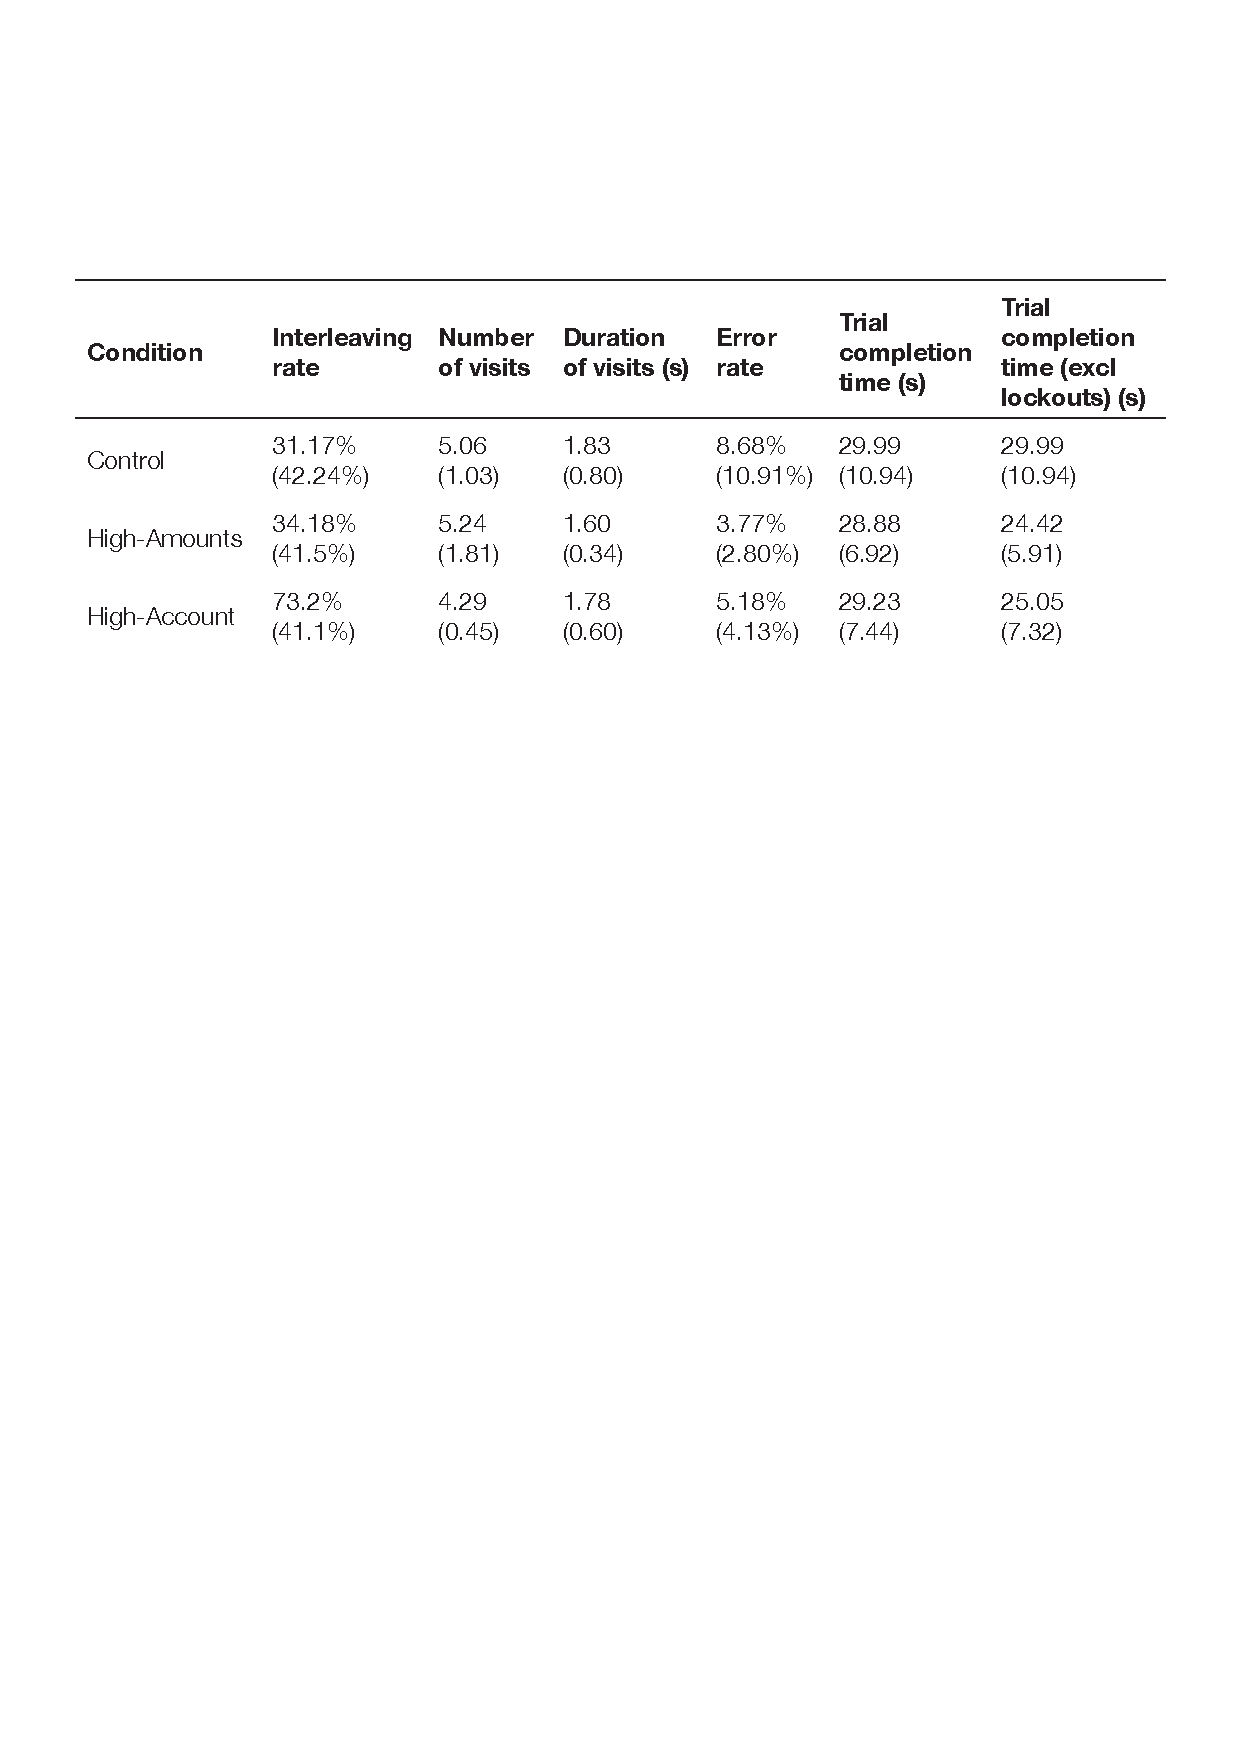
\includegraphics[width=\textwidth]{images/ch34/ch34-means.pdf}
\caption{The means (and standard deviations) of all dependent measures for each condition. The rates are calculated by dividing the number of occurrences to the number of opportunities, e.g. an interleaving rate of 50 percent means participants interleaved on 50 percent of trials.}
\label{tbl:ch34_4-means}
\end{table}

\subsubsection{Interleaving strategies}
A trial was labelled as 'interleaving' if the participant started entering one expense but interleaved to the other expense before completing the first one. The interleaving rate for each condition was calculated by dividing the number of trials where people interleaved by the number of total trials. 

The boxplots in Figure \ref{fig:ch34_4-boxplots} show the variability of interleaving rates across conditions. The Control condition had a median interleaving rate of 6\%, the High-Amount conditions had a median interleaving rate of 12\%, and the High-Account condition had a median interleaving rate of 96\%.

\begin{figure}
 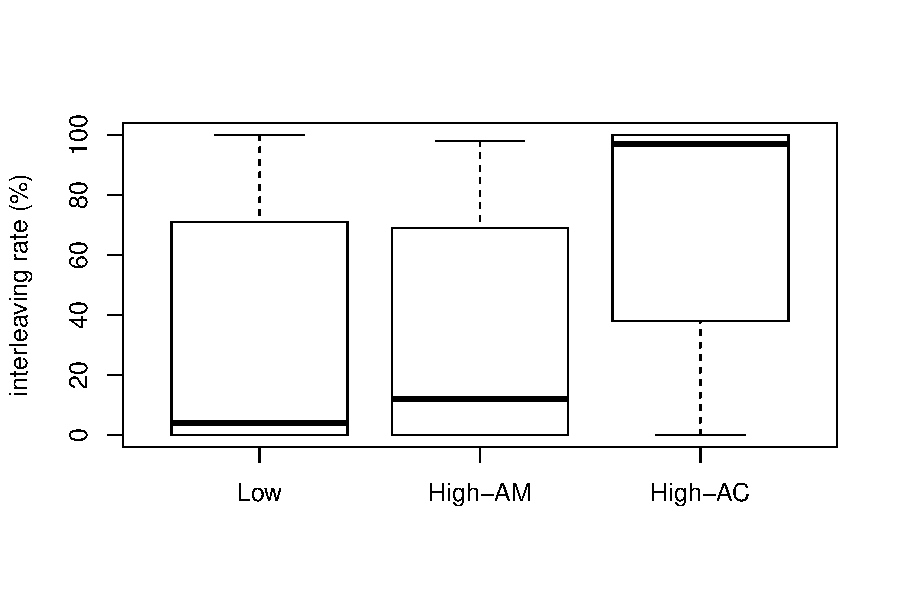
\includegraphics[width=0.6\textwidth]{images/ch34/ch4_4-boxplot.pdf}
\caption{Boxplot of interleaving rates in each condition.}
\label{fig:ch34_4-boxplots}
\end{figure}

\begin{figure}
 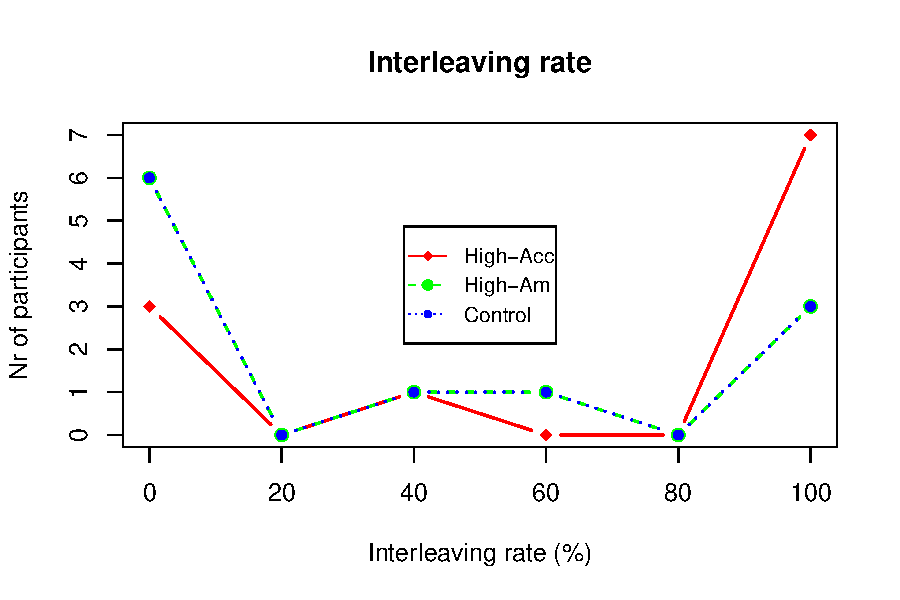
\includegraphics[width=\textwidth]{images/ch34/ch34-4_linechart.pdf}
\caption{Line graph showing the frequency of interleaving rates for each condition. As can be seen, all three lines have two peaks at 0 and 1, which means that most participants interleaved on 0\% or 100\% of all trials.}
\label{fig:ch34_4-linechart}
\end{figure}

Participants interleaved most often between expenses in the High-Account condition (M = 73.2\%, SD = 41.1\%), compared to the Control (M = 31.17\%, SD = 42.24\%) and High Amount (M = 34.18\%, SD = 41.5\% ) conditions, $\chi^2$(2) = 6.81, p = 0.03. A post-hoc Dunn's test showed there was a difference between the High-Account condition and the Control (p = 0.02) and the High-Amount p = 0.03) conditions, but not between the Control and High-Amount conditions (p=0.9).

In the High-Account condition, participants predominantly switched to the page with the Amounts first, which had no time delay, and entered these into the data entry form. In the other two conditions, participants mostly entered an amount and account code of the first expense first, and then entered the amount and account code of the second row. 

Across conditions, most participants were consistent in their strategy choice, and either interleaved between expenses on almost no (0\%) or all (100\%) trials. This is illustrated in Figure \ref{fig:ch34_4-linechart}, which shows the distribution of interleaving rates for each condition. The lines all have peaks at the left and right end, indicating the interleaving rate was predominantly 0 or 100\% in each condition.

The consistency in strategy choice is further illustrated in Figure \ref{fig:ch34_4-plotpp}, which displays a plot for each participant across trials. The x axis plots the trial number, and the y axis displays whether they interleaved on that trial or not: a value of 0 means they did not interleave, and a value of 1 means they did interleave. These plots further illustrate that most participants were consistent in interleaving on no or all trials (see for example Participant 6, who interleaved on all trials). A subset of participants switched between strategies at the first couple of trials before sticking with one strategy, such as Participants 9 and 12. Lastly, participants 29, 32 and 33 seemed to switch between the strategies throughout the experiment and did not stick with a particular strategy.

\begin{figure}[!htbp]
    \centering
    \begin{subfigure}[b]{0.5\textwidth}
        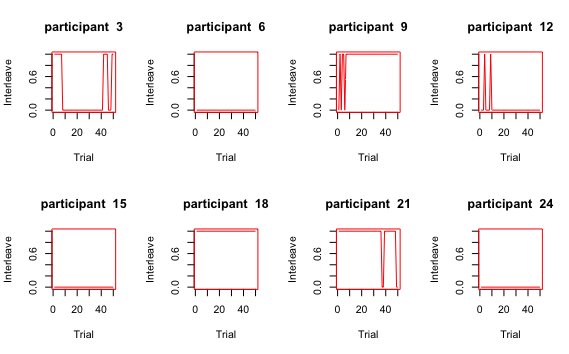
\includegraphics[width=\textwidth]{images/ch34/ch34-4_plotControl(1).png}
        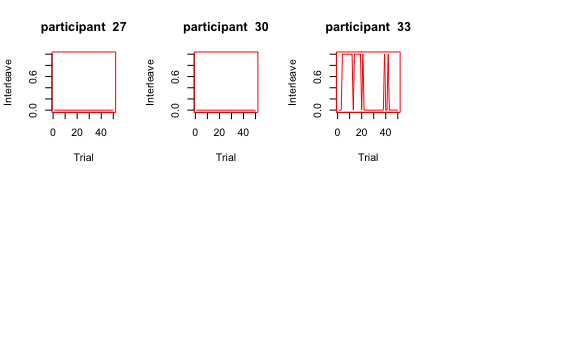
\includegraphics[width=\textwidth]{images/ch34/ch34-4_plotControl(2).png}
        \caption{Participants in the Control condition.}
    \end{subfigure}
    ~ %add desired spacing between images, e. g. ~, \quad, \qquad, \hfill etc. 
      %(or a blank line to force the subfigure onto a new line)
    \begin{subfigure}[b]{0.5\textwidth}
        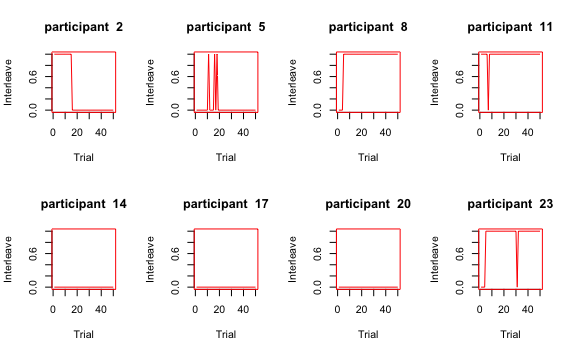
\includegraphics[width=\textwidth]{images/ch34/ch34-4_plotHigh-Am(1).png}
         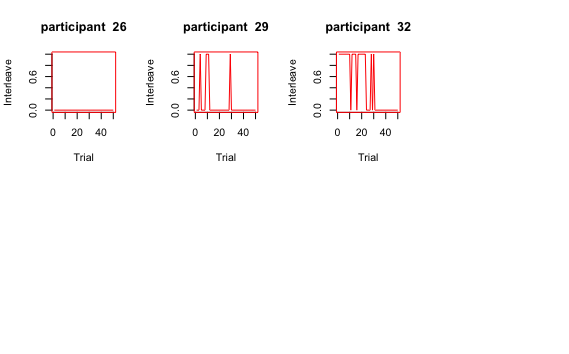
\includegraphics[width=\textwidth]{images/ch34/ch34-4_plotHigh-Am(2).png}
        \caption{Participants in the High-Amount condition.}
    \end{subfigure}
        \begin{subfigure}[b]{0.5\textwidth}
        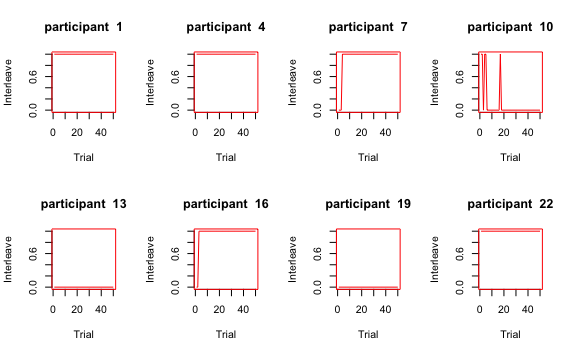
\includegraphics[width=\textwidth]{images/ch34/ch34-4_plotHigh-Acc(1).png}
         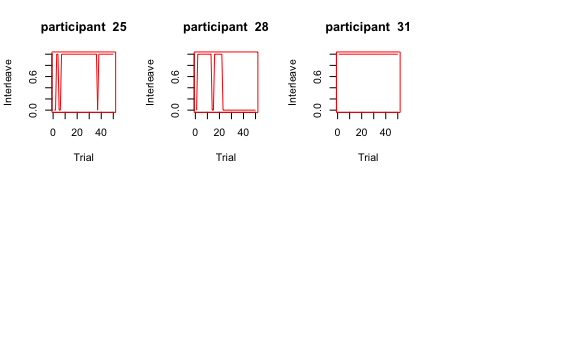
\includegraphics[width=\textwidth]{images/ch34/ch34-4_plotHigh-Acc(2).png}
        \caption{Participants in the High-Account condition.}
    \end{subfigure}
    ~ %add desired spacing between images, e. g. ~, \quad, \qquad, \hfill etc. 
    %(or a blank line to force the subfigure onto a new line)
    \caption{A plot per participant across trials. The x axis shows the trial number, and the y axis indicates whether a participant interleaved on a trial: a value of 0 means they did not interleave, a value of 1 means they did interleave.}\label{fig:ch34_4-plotpp}
\end{figure}

\subsubsection{Number and duration of visits}
There was no difference in the number of visits, $\chi^2$(2) = 2.90, p = 0.23. On average, participants made 4 visits per trial (i.e. one visit per data entry). Participants visited an information page for 1.8 seconds on average, and there was no significant difference in duration of visits between conditions, $\chi^2$(2) = 0.30 p= 0.8. 

To get a better insight in the specific order in which participants viewed and entered items, the trials were grouped based on the order of actions. There were eight different possible actions: viewing the first amount (V-Am1), viewing the second amount (V-Am2), viewing the first account code (V-Acc1), viewing the second account code (V-Acc2), entering the first amount (E-Am1), entering the second amount (E-Am2), entering the first account code (E-Acc1), and entering the second account code (E-Acc2). This iteration of grouping the trials resulted in 17 different strategy groups in total, with the majority of trials (98\%) grouped in the same four groups, which are shown in Figure \ref{fig:ch34_4-groupstr}. For example, the first strategy (a) shows a strategy where participants started a trial by visiting the Amount page, and then visiting the Accounts page. They then entered both the amounts of the first expense (Am1) and the account code of the first expense (Acc1). They then visited the Amounts page again, and entered the amount of the second expense (Am2), and then visited the Accounts page again and entered the account code of the second expense (Acc2). Table \ref{tbl:ch34_4-groupstr} shows the frequency with which these strategies were chosen per condition.

\begin{figure}[!ht]
  \centering
    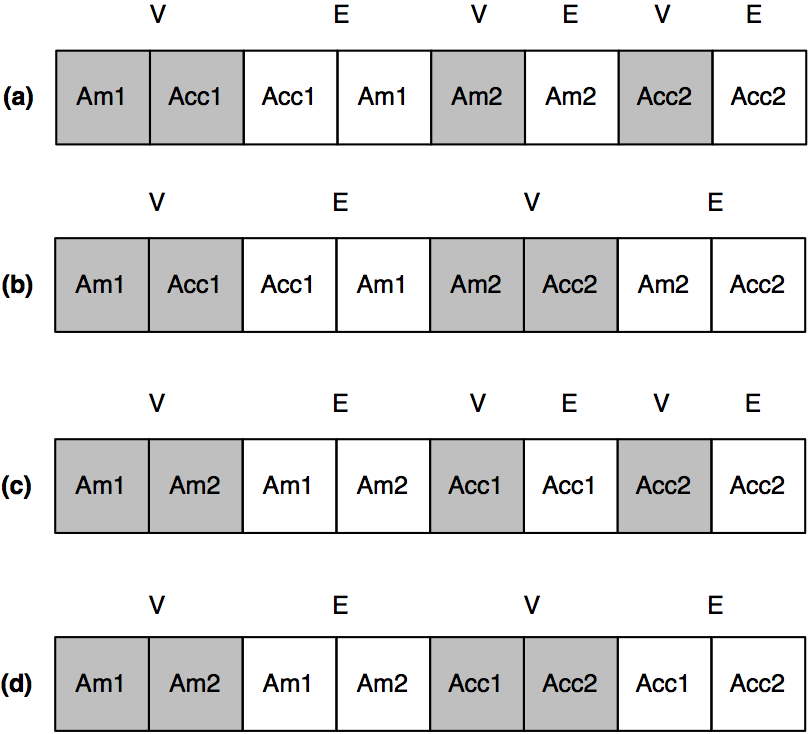
\includegraphics[width=0.5\textwidth]{images/ch34/ch34_4-groupstr.png}
      \caption{The sequence of the most common grouping strategies. V = visit to the data source, E = entry of the data item. For example, in Strategy (a) a participant first viewed Amount1 and Account1, and then entered Amount1 and Account1. He/she then viewed Amount2 and entered it, and then viewed Account2 and entered it.}
          \label{fig:ch34_4-groupstr}
\end{figure}

\begin{table}[!ht]
\centering
\resizebox{\textwidth}{!}{
\begin{tabular}{l|l|l|l|l|ll}
\cline{2-5}
                                   & \multicolumn{2}{l|}{Row}                                                      & \multicolumn{2}{l|}{Column}                                                    &                                  &                                \\ \hline
\multicolumn{1}{|l|}{Condition}    & First row (a)     & \begin{tabular}[c]{@{}l@{}}First \&\\ Second row (b) \end{tabular} & Amounts (c)       & \begin{tabular}[c]{@{}l@{}}Amounts \& \\ Accounts (d) \end{tabular} & \multicolumn{1}{l|}{Other}       & \multicolumn{1}{l|}{Total}     \\ \hline
\multicolumn{1}{|l|}{High-Account} & 34\%  {\footnotesize (48)}     & 4\%  {\footnotesize (6)}                                                       & 57\%  {\footnotesize (80)}     & 2\%  {\footnotesize (3)}                                                        & \multicolumn{1}{l|}{3\%  {\footnotesize (4)}}     & \multicolumn{1}{l|}{100  {\footnotesize (141)}} \\ \hline
\multicolumn{1}{|l|}{High-Amount}  & 20.99\%  {\footnotesize (44)}  & 16.57\%  {\footnotesize (35)}                                                  & 49.72\%  {\footnotesize (104)} & 9.39\% {\footnotesize  (20)}                                                    & \multicolumn{1}{l|}{3.31\%  {\footnotesize (7)}}  & \multicolumn{1}{l|}{100  {\footnotesize (210)}} \\ \hline
\multicolumn{1}{|l|}{Control}      & 11.2\%  {\footnotesize (16)}   & 21.6\%  {\footnotesize (32)}                                                   & 54.4  {\footnotesize (81)}     & 12\%  {\footnotesize (18) }                                                     & \multicolumn{1}{l|}{0.8\%  {\footnotesize (1)}}     & \multicolumn{1}{l|}{100  {\footnotesize (148)}} \\ \hline
\multicolumn{1}{|l|}{Total}        & 21.18\%  {\footnotesize (190)} & 15.02\%  {\footnotesize (73)}                                                  & 52.96\%  {\footnotesize (265)} & 8.37\%  {\footnotesize (41)}                                                    & \multicolumn{1}{l|}{2.46\% (12)} & \multicolumn{1}{l|}{100  {\footnotesize (499)}} \\ \hline
\end{tabular}
}
\caption{The most common grouping strategy was to chunk the items into three groups. The strategies are shown graphically in Figure \ref{fig:ch34_4-groupstr}.}\label{tbl:ch34_4-groupstr}
\end{table}


\subsubsection{Errors and trial completion time}
There were 200 data entries, so in total there were 200 opportunities for a participant to make a data entry error. The error rates were calculated as the number of errors divided by the number of entries. Though the mean error rate was higher in the Control condition (M=8.68\%, SD=10.90\%) compared to the High-Amount (M=3.77\%, SD=2.79\%) and High-Account (M=5.18\%, SD=4.13\%) conditions, this difference was not statistically significant, $\chi^2$(2) = 0.41, p = 0.8. 
The High-IAC conditions already had an extra time cost to overall completion time, due to the delay to one of the pages. Therefore, two completion times were calculated: one of the actual completion time, which included the lockout times, and another with these times removed. Considering these two times, there was no difference in the time it took to complete a trial using the actual completion time, X(2) = 0.15, p= 0.9, and with the lockout times removed,  $\chi^2$(2) = 2.92, p = 0.2. On average, participants took about 29 seconds per trial across conditions.

\citet{Wiseman2011} taxonomy of number entry errors was used to analyse the types of data entry errors that were made. As can be seen in Figure x , the most prominent error types were when participants had a digit(s) wrong (60 times), when a data entry was skipped (75 times) or when they entered a correct number, but in the wrong input field (57 times): these types of errors make up for 61\% of all errors.


\subsubsection{Qualitative findings}
After the experiment had ended, participants were debriefed and the purpose of the study was explained. Some participants recalled their strategies and gave additional explanations behind them.

x participants adapted their strategy several times throughout the experiment, in order to find the quickest way to complete the task. Because amounts were shorter and easier to remember, several participants mentioned they tried to first view all amounts before entering them. They tried this strategy with account codes as well, but these were longer and therefore it was more difficult to memorise two at a time. As. a result, most participants ended up viewing and entering each account code one by one.

Several participants noticed that numbers re-occurred throughout the experiment. They felt it was easier to memorise a number that had already occurred earlier in the experiment, so when a trial contained a number they had entered before, they would use the 'Grouped' strategy: they viewed another window and item before returning to the entry form. Furthermore, some participants started a trial by not viewing any other windows, but re-entering the data items of the previous trial in the data entry form. They would then visit the information source windows to check if the items were the same, or if they needed to change some of the items.

\subsection{Discussion}
%Summary
The aim of this study was to investigate the effect of IAC on how people manage task interruptions to look up information from multiple information sources with varying IACs. IAC influenced the order in which people entered data, and whether and how they chunked data items. 
In the Control condition, when there were no differences in IAC, participants tended to complete a data entry sheet in sequential order, and completed one expense before moving to the next one. When comparing this with the High-IAC conditions, people interleaved significantly more between expenses in the High-Account but not High-Amount condition. These findings partly support the hypothesis that people postpone looking up information with a higher IAC, but it does not account for why people continued to enter the sheet in sequential order in the High-Amount condition. 

%Why would people continue to do it one by one if there is an added cost?
These results can be explained when considering the order in which the data was presented, and the order in which items were entered. Across conditions, participants predominantly started each trial by entering the first cell of the data entry sheet, the amount of the first expense, regardless of whether the Amounts page had a 2-s delay. However, the second item they entered was dependent upon which window had a delay: if the amounts window had a delay, they would enter the account code first. If there was a delay with the accounts, they would enter the second amount first.
It seems that IAC does not influence the first visit, but does affect subsequent visits. Even though the IAC was consistent throughout the experiment, potentially the experiment was too short for participants to learn which of the windows had a delay and only adapted their strategy after they had already entered the first item. Furthermore, participants tended to stick to the same strategy they had started with throughout the experiment. We will discuss this result further in the General Discussion.

In Experiment 1, both expenses were shown on the same page, and could be seen as part of the same task. We wonder whether differences in IAC also makes people interleave between two distinct tasks, which are shown on separate pages. The aim of the next experiment was therefore to study the effect of differences in IAC in a multi-task setup.



%ORDERING STRATEGIES
\subsubsection{Ordering strategies}
%\item[RQ2.] \textit{How does IAC affect the order of visits to look up information from multiple sources with different IACs?}
%\item [H2.]As the experiment progresses and people become aware how costly it is to access certain sources, they will learn and choose to enter all the Low-IAC items first, in a batch, and then the High-IAC items second, also in a batch, rather than looking up each item as they need it. 

IAC had an effect on people's ordering strategies, but only in the condition where the IAC was increased for accessing account codes. People first looked up and entered the low IAC items, the amounts, before they entered the high IAC items, the account codes. However, if the cost to access the amounts was increased, people entered items row by row, as participants did in the control condition.

In \citet{OHara1998}'s study on the effect of IAC on problem solving tasks, participants in Low-IAC and High-IAC conditions initially performed the same type of strategies. However, over time participants in a High-IAC condition  learnt more efficient strategies, whilst participants in a Low-IAC condition continued to use the same strategy. Prior work has also shown that people who are exposed to High-IAC situations will adopt and continue to use a certain strategy, even in situations where the cost to access information is no longer high \citep{Patrick2014}. It is therefore expected that once participants learn it is more efficient to group high-IAC items, they may adopt this strategy for low-IAC items as well. In Study 2 of this thesis, people tried to enter items that were nearby in the environment first, and postponed looking up other information until later. Based on these findings, the following hypothesis is made: 

In previous studies, people would postpone or not address information needs if there was a high time cost associated with it \citep{Sohn2008}. This was also found in Study 2. People initially tried to do tasks as they needed it, but if it took too long, they would put it aside.

In the current study, this was also found but the cost to memorise an item overrode the cost to access it: people would first enter the amounts, even if the cost to access them was higher.
If the cost was high, they would try and memorise them both before entering them. This shows people try to minimise interleaving between viewing and entering information. 

%GROUPING STRATEGIES
\subsubsection{Grouping strategies}
%\item[RQ1.] \textit{How does IAC affect the number of visits to look up information from multiple sources with different IACs?}
%\item[H1.]As IAC increases, people will try to group and memorise multiple items to minimise visits.

The soft constraints hypothesis predicts that people choose and adapt their task strategies in order to minimise time \citep{Gray2006}. Study 3 found that the longer it takes to access information, the more items people try to memorise in one visit. Based on these findings, the following hypothesis is made: 

%GROUPING STRATEGIES
\subsubsection{Performance}
%\item[RQ3.] \textit{Do the number and order of visits affect data entry accuracy and speed?}

\subsubsection{Grouping strategies}
IAC also had an effect on how often people switched between visiting and entering information. In the conditions where the amounts were low, people often visited multiple items before returning to the entry interface. Though there was no difference in errors in the current study, it can be imagined this strategy is more risky as people are away for longer so resuming a task is more difficult, and they are storing more information in memory, so people may misremember information.

In the condition where the IAC for amounts was high, this strategy was not used as frequently. 
IAC thus does not have to be bad if the information is easy enough to briefly hold in memory (condition amounts high).

IAC made people changes strategies even if only two of the four information sources had an increased IAC. This is in accordance with \citep{Morgan2014}, who showed that a more memory-based strategy can be trained for future situations. When people were exposed to an interface with an increased access cost, they adopted a memory-based strategy and retained this strategy, even when they then interacted with an interface with lower access costs.


\subsubsection{Conclusion}
This study investigated the effect of IAC on looking up information from multiple sources, and showed that, if all information has the same IAC it is better if this is low, differences in IAC between sources can make people schedule their subtasks more efficiently and effectively. People needed less visits and made fewer errors. 
However, for this study people only had one data entry task at a time to focus on, and the sources only contained information for this single task. In Study 1 and 2, people often batched and saved up multiple data entry tasks, and sources included more than just the information for one task: for example, if people had to look up an account code, this was often retrieved from a spreadsheet with all account codes. They thus not only had to manage subtasks of one data entry task, but had to coordinate multiple data entry tasks. In order to save visits, people may therefore look up information for several tasks and interleave. One of the participants from Study 1 shared that this did occur and said she and colleagues had to be very careful to not input information in the wrong form. If people group information subtasks per IAC for a single task, would they also group these subtasks per IAC when dealing with multiple tasks? In order to answer this question, a follow-up study was run to see the effect of IAC on interleaving behaviour between two claim forms. 

\section{Study 5: Interleaving between data entry tasks}
 
\subsection{Introduction}
Study 4 showed that people group subtasks of looking up information according to the information's IAC: if all information sources were equally easy to access, participants looked up and entered information for a task in sequential order. However, if some sources were more costly to retrieve, people first retrieved and entered all low IAC items, before they retrieved high IAC items.
If people deal with multiple data entry tasks, would this also make people more likely to look up and enter low IAC items across tasks, rather than completing one task at a time? 
In Study 2, participants saved up data entry tasks to do in one session and occasionally had multiple data entry tasks open at the same time. Multitasking between data entry tasks is a common occurrence, but this strategy can be prone to errors.
The aim of the current follow-up study is to see if differences in IAC between information sources makes people more likely to interleave between data entry tasks.

The following question will be addressed:

What is the influence of IAC on interleaving between data entry tasks?

\subsection{Method}
\subsubsection{Participants}
Fourty-two participants (32 female), ranging from 18-46 years (M = 25, SD= 8) took part in the experiment. They were recruited from a university subject pool and received $\pounds$4 for their participation.

\subsubsection{Materials}
The task was similar to the one used in Study 4 but differed in one aspect. Instead of filling in one data entry form per trial, participants had to complete two forms per trial, which were shown on two different pages (see Figure \ref{fig:ch34_5-tasklayout}.Each data entry sheet contained one expense, and participants completed the trial by entering the amount and account code for each sheet. The aim of this follow-up study was to investigate if differences in IAC of the two sources makes people more likely to interleave between two separate data entry tasks.

\begin{figure}
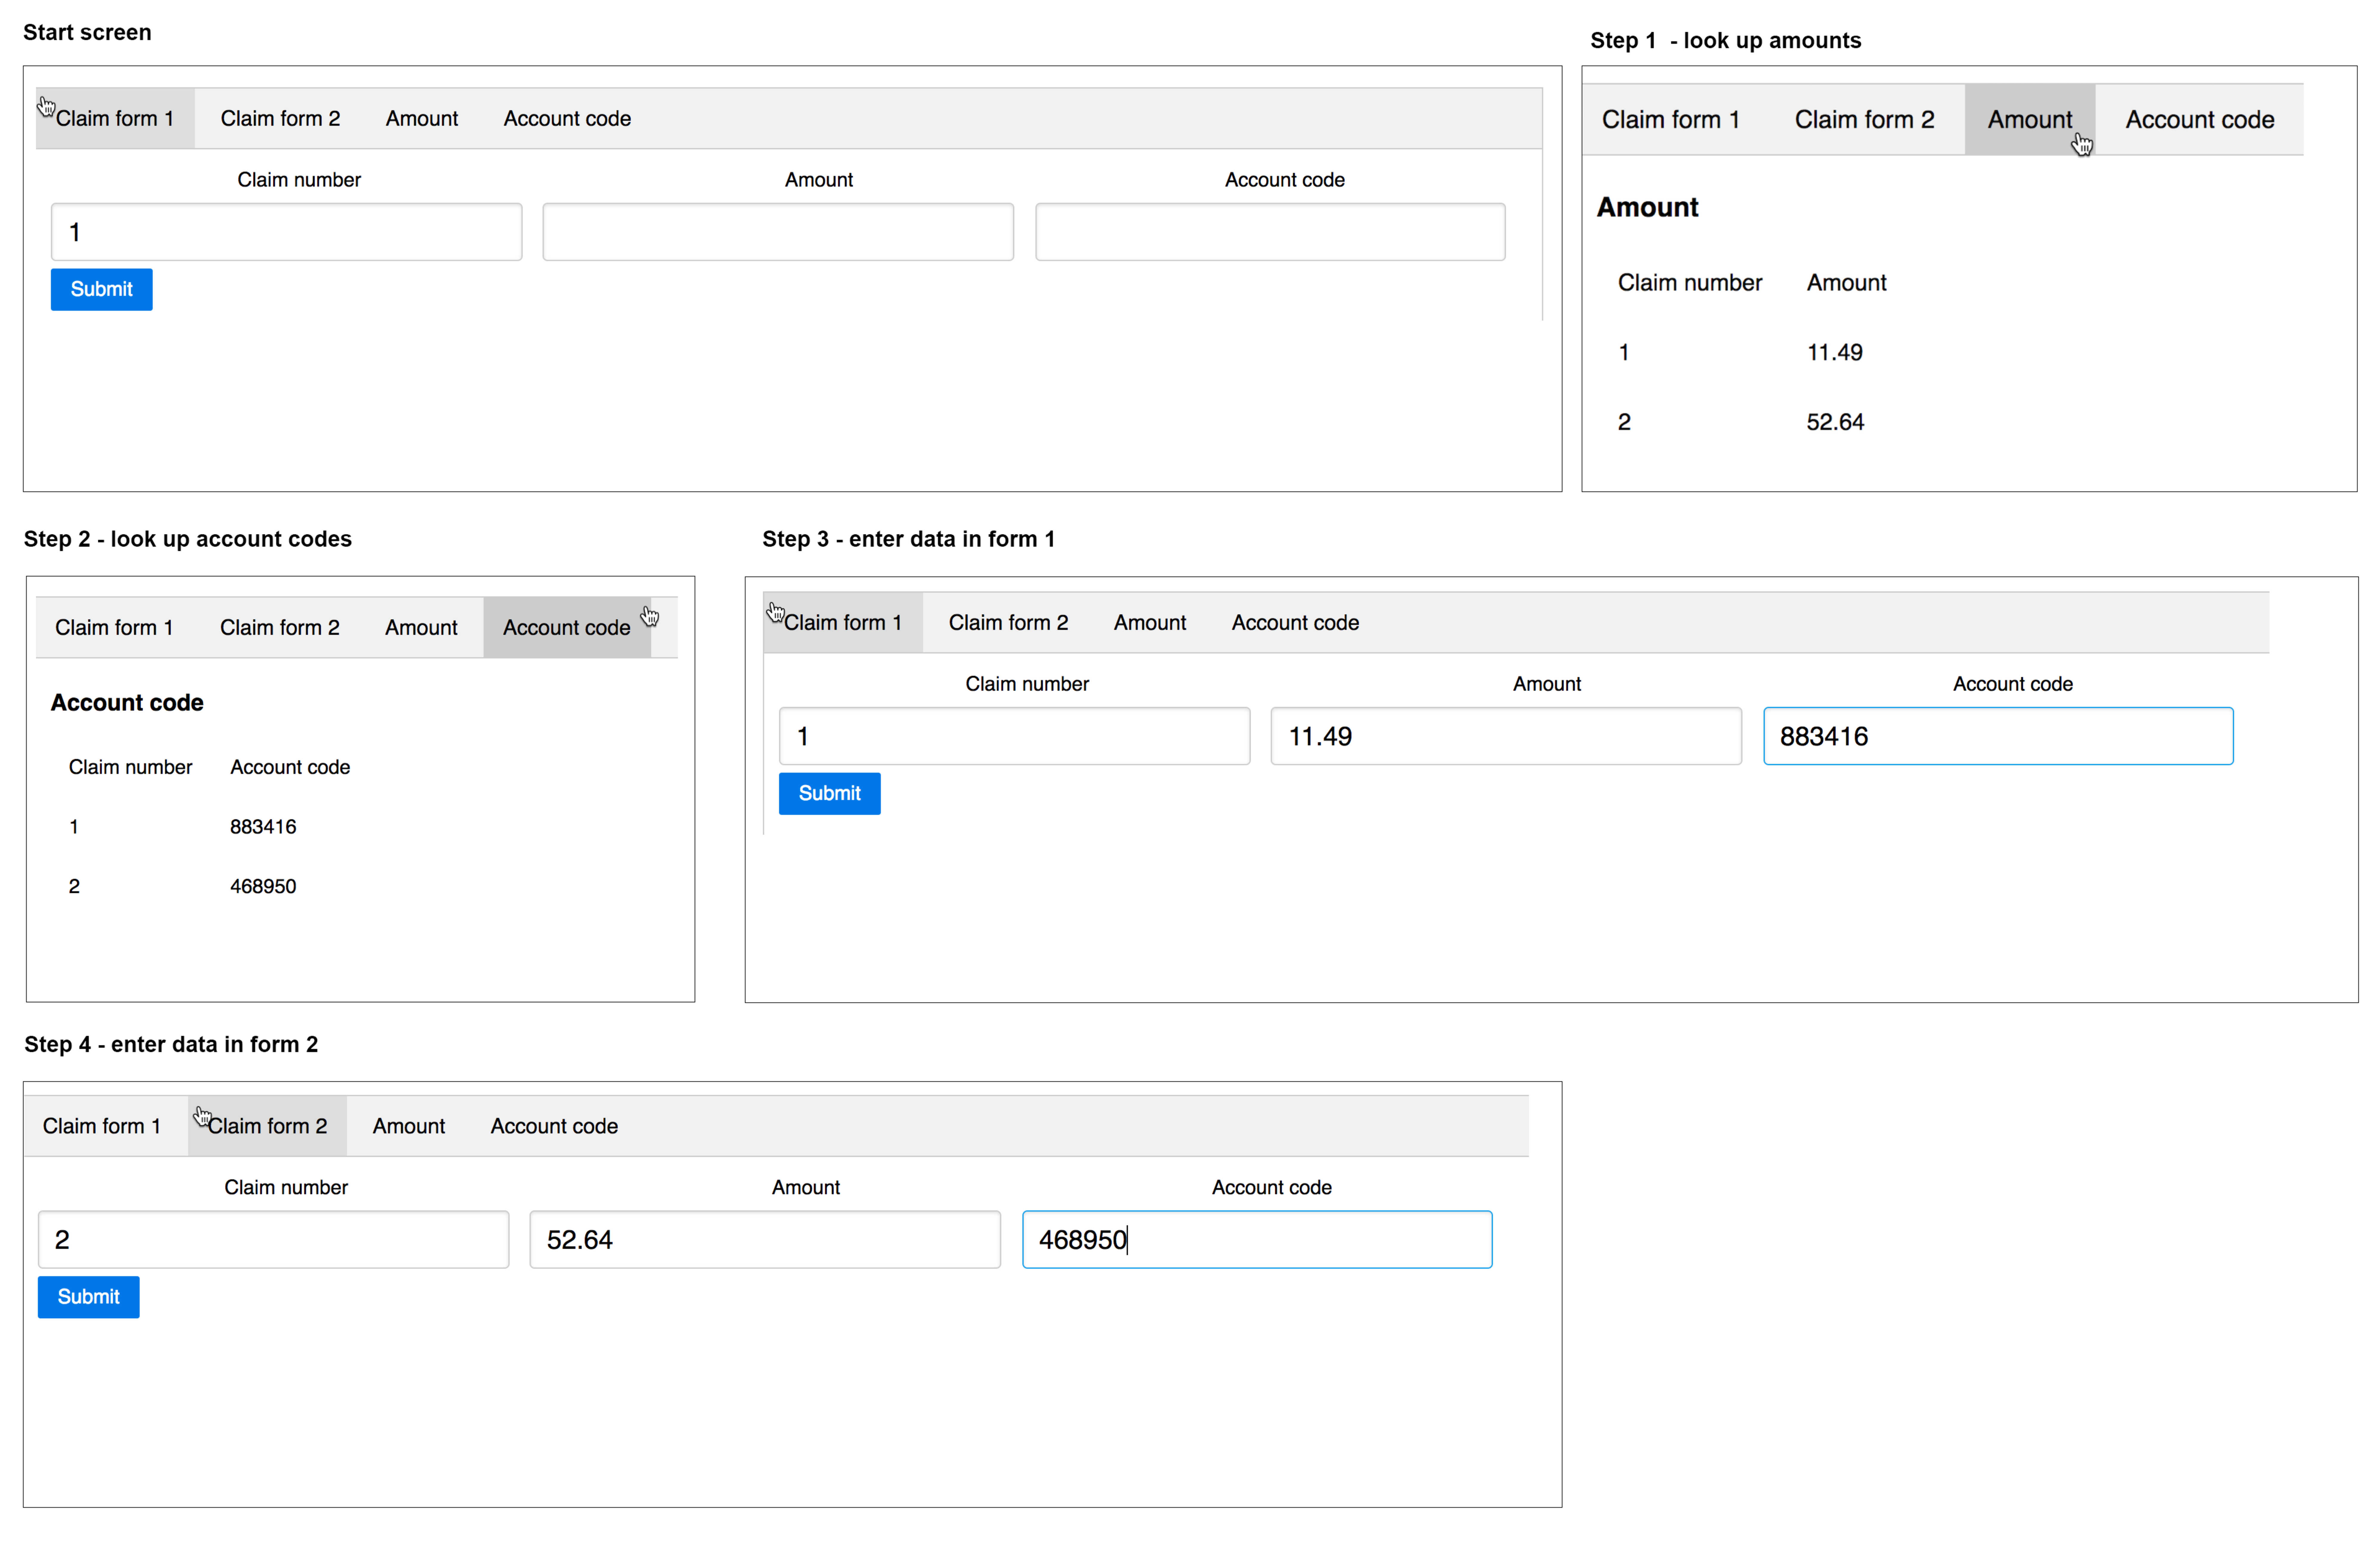
\includegraphics[width=\textwidth]{images/ch34/ch34-5_Tasksequence.pdf}
    \caption{Participants had to enter two data entry forms per trial, each containing two items. Each trial started by showing the first data entry form. As in Study 4, the data items for both forms were retrieved from a separate Amounts page (Step 1) and an Accounts page (Step 2). Participants had to enter the items for the first form (Step 3) and second form (Step 4) before submitting the data entries and moving on to the next trial.}\label{fig:ch34_5-tasklayout}
\end{figure}

\subsubsection{Design}

The experiment was a between-participants design with the presence of a delay as the independent variable. As in Study 4, in the Control condition there were no delays in opening the pages. In the High-Amount condition, there was a delay in opening the page with amounts. In the High-Account condition, there was a delay in opening the page with account codes. The main dependent variable was whether participants interleaved between sheets or not: did participants enter the data items in sequential order, or did they interleave between the two sheets? If participants entered the amount and account code of one sheet before entering the other sheet, this was considered a sequential order. If participants entered amounts of each sheet first, followed by entering the account codes or vice versa, this was considered interleaving. All key presses were recorded to determine in which order data was entered. Page switches were recorded to capture when and how often a participant looked up the data items. Other dependent variables were trial completion time, data entry error rate, and type of errors.

\subsubsection{Procedure}
The experimental setup was similar to Study 4. For each experimental trial, participants had to enter four data items: they had to complete two forms with two entries each, an account code and an amount. For each experimental trial, participants had to enter four data items, two for each sheet. It was explained that they could use any strategy they wanted, but that it was important to complete both sheets before continuing to the next trial. Participants first completed two practice trials to familiarise themselves with the task, and data from the practice trials were excluded from the analysis. The experiment took approximately 30 minutes.

\subsection{Results}
Three participants were removed from the data due to extreme values on performance measures.
P28 and P23 made at least one error on every trial. They made 118 and 153 errors out of 200 error opportunities, respectively. P26's session was terminated before the end had been reached, as 45 minutes had passed. This participant spent on average 65 seconds per trial, which is twice as long as the mean trial time of other participants.

These three participants were considered outliers and removed from the data. Data of the remaining 39 participants was taken into the data analysis.

Table \ref{tbl:ch34_5-means} shows a summary of the results of all three conditions for the dependent variables. Kruskal-Wallis tests were carried out to test if there were significant differences between the conditions.

\begin{table}
 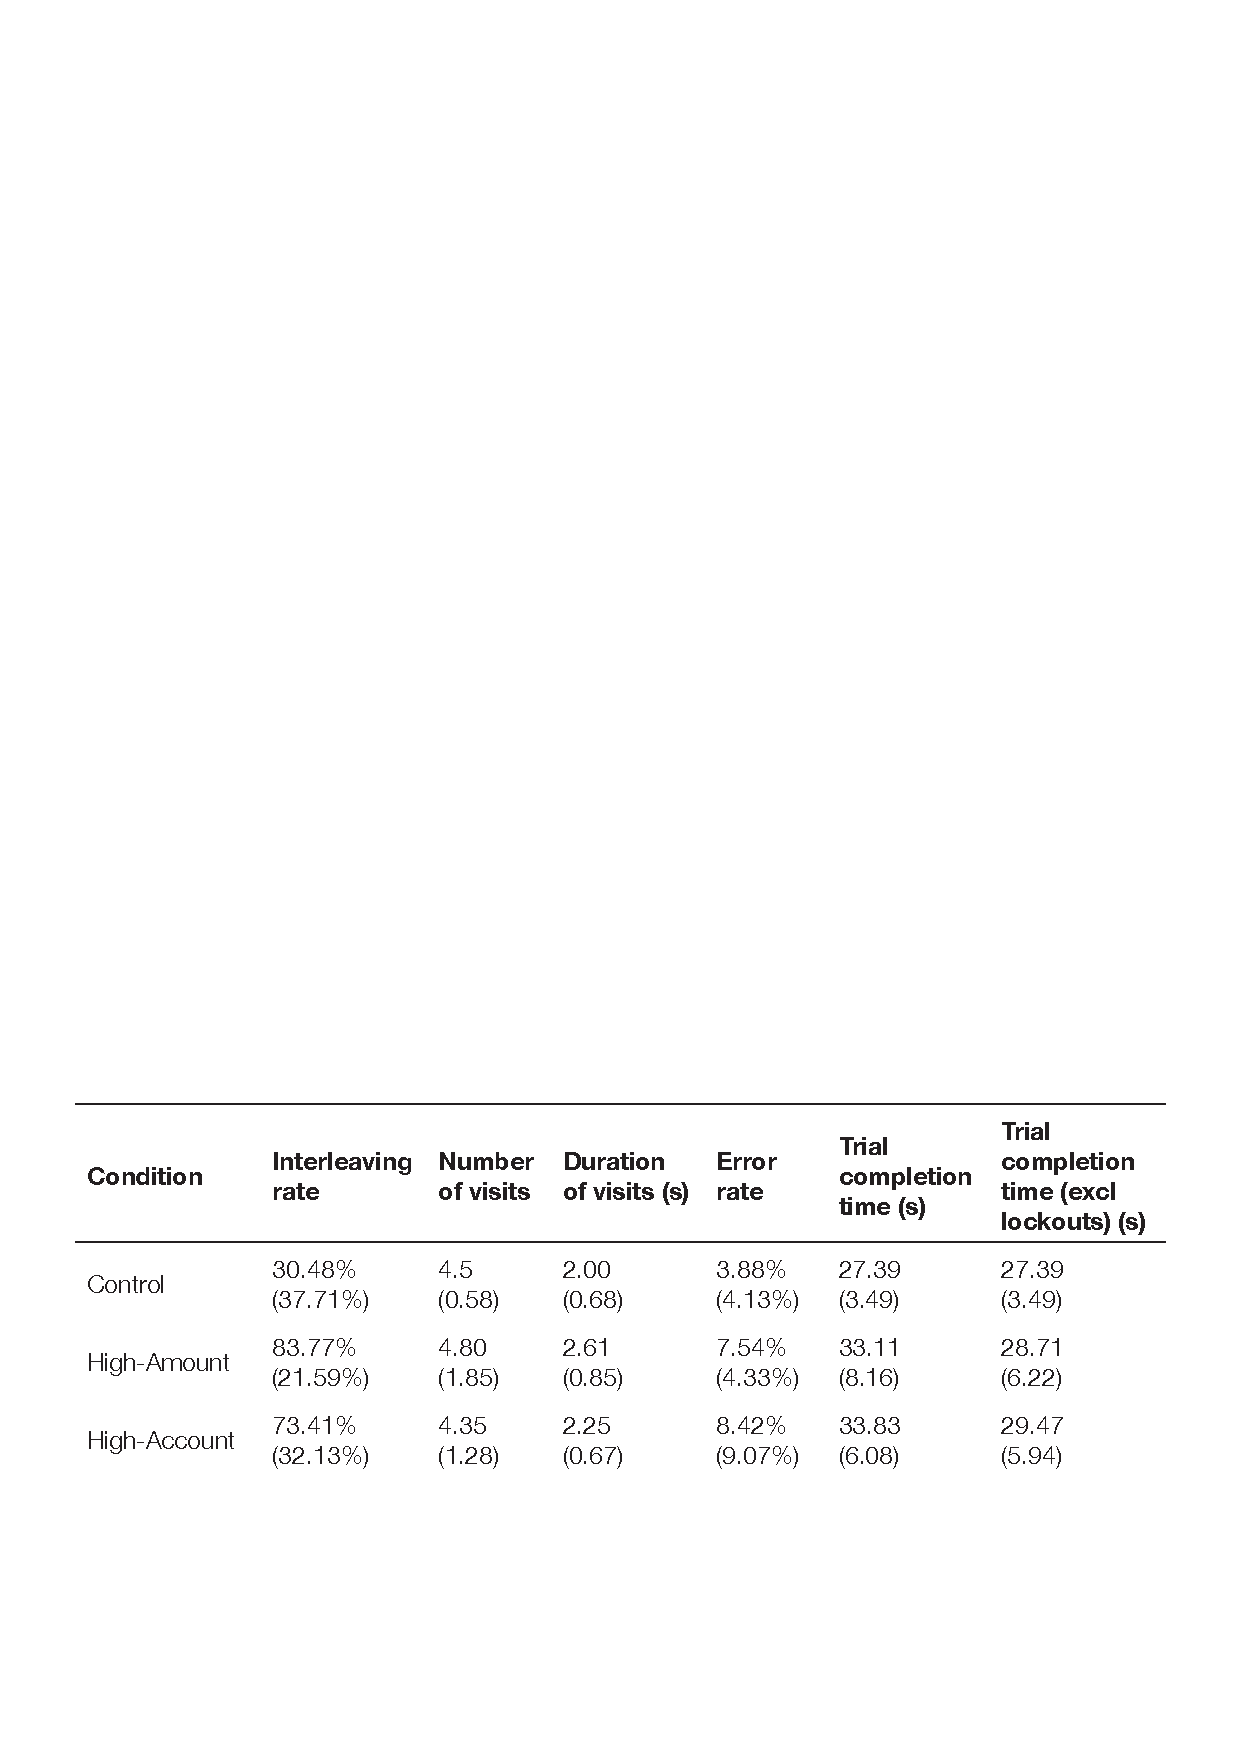
\includegraphics[width=\textwidth]{images/ch34/ch34_5-means.pdf}
\caption{The means (and standard deviations) of all dependent measures for each condition. The rates are calculated by dividing the number of occurrences to the number of opportunities, e.g. an interleaving rate of 50 percent means participants interleaved on 50 percent of trials.}
\label{tbl:ch34_5-means}
\end{table}

\subsubsection{Interleaving strategies}
A trial was labelled as 'interleaving' if the participant started entering one data entry sheet, but interleaved to entering items on the other sheet before completing the first one. The interleaving rate for each condition was calculated by dividing the number of trials where people interleaved by the number of total trials. 

The boxplots in Figure 4 show the variability of interleaving rates across conditions. Participants interleaved most often between data entry sheets in the High-Account (M = 73.4\%, SD = 32.1\%) and High Amount (M = 83.8\%, SD = 21.6\% ) conditions compared to the Control (M = 30.5\%, SD = 37.7\%) condition, $\chi^2$(2) = 11.13, p = 0.004. A post-hoc comparison showed there was a differnece between the Control and the High-Amount (p<.01) and High-Account (p = 0.01) conditions, and no difference between the High-Account condition and the High-Amount (W = 22, p = 0.4) conditions.

As can be seen in Figure x, which shows the distribution of interleaving rates, all participants in the High-IAC conditions interleaved on at least a part of the trials. This is illustrated by the left side of the graph: the lines of the High-IAC conditions have a frequency of 0 participants at an interleaving rate of 0\%. The Control condition line has no obvious peak, indicating that interleaving rates in this condition were evenly distributed: participants interleaved on zero, a portion, as well as all of the trials.

As in Study 1, participants made on average four visits per trial, i.e. one visit per data entry. There was no difference in the number of visits, $\chi^2$(2) = 1.59, p = 0.5. Participants made significantly shorter visits in the Control (M = 2.00s, SD = 0.68s) condition compared to the High-Account condition (M = 2.25s, SD = 0.67s) compared to the High-Amount (M = 2.61s, SD = 0.85s) and  $\chi^2$(2) = 6.14, p= 0.04. Post-hoc comparisons found a significant difference between  the High-Amount and the Control (p=.02) conditions, but not between High-Account and Control conditions (p = 0.2) or the High-Account and the High-Amount (p = 0.2).

%Participants' data entry strategies were categorised in one of two categories: they either interleaved between the two data entry forms (e.g. entering amount on Form1, followed by entering the amount in Form 2), or they filled the forms in sequential order (entering amount and account code on Form1, followed by entering the amount and account code on Form2).
%
%Table \ref{table:ch34_Study5interleavingfreqtbl} shows the frequency of strategies per condition. In total, the strategy was chosen on 333 trials in the High-Account condition, 427 trials in the High-Amount condition, and 184 trials in the Control condition. In other words, the strategy was chosen on 66.6\%, 85.4\% and 40.88\% of the trials, respectively.  There was a significant difference in interleaving behaviour,
%F(2,30) = 4.41, p = .02. A post-hoc comparison showed people interleaved significantly more often in the High-IAC conditions than the Control condition  (p = 0.02) . There was no significant difference between the High-Account and High-Amount condition (p = 0.18).

%A Kruskal-Wallis test shows there is a significant difference between the different conditions,  $\chi^2$ (2, N = 29) = 6.68, p = 0.035. Mann-Whitney U tests were used to get further insight in pairwise differences between conditions. Participants interleaved significantly more often in the High-IAC conditions than the Control condition  (U = 138, p = 0.02) . There is no significant difference between the High-Account and High-Amount condition (U = 32, p = 0.18).

%A chi-square test shows that the frequency of interleaving strategy was significantly associated with the condition, $\chi^2$  (2) = 207.29, p= < 0.05.


\subsubsection{Errors and trial completion time}
There were 200 data entries, so in total there were 200 opportunities for a participant to make a data entry error. The error rates were calculated as the number of errors divided by the number of entries. 
There was a marginal though not significant effect of IAC on error rate, $\chi^2$(2) = 5.37, p = 0.06. The mean error rate was marginally higher in the High-Account condition (M= 8.42\%, SD=9.08\%) compared with the High-Amount (M=7.54\%, SD=4.33\%) and Control (M=3.88\%, SD=4.13\%) conditions. When comparing the actual completion time including lockouts, participants were significantly faster in the Control condition (M=27.39, SD = 3.49s) than the High-Account (M = 33.83s, SD = 6.08s) or High-Amount (M = 33.11s, SD = 8.16s) conditions,  $\chi^2$(2) = 8.52, p= 0.01. With the lockout times removed, the difference is no longer significant, $\chi^2$(2) = 1.61, p = 0.4.

The type of errors can be seen in Figure. The most common error type was when a data entry was skipped: this happened 243 times. Table 1 shows the number of skipped errors for each condition. It can be seen that in the Control condition this type of error occurred 16 times. The error happened more frequently in the High-IAC conditions: in the High-Account condition it happened 114 times, and in the High-Amount condition it happened 116 times.
Typing the correct number but in the wrong field happened 78 times. This happened 18 times in the Control condition, 14 times in the High-Account and 46 times in the High-Amount condition.
When comparing across conditions, these types of errors happened on a significantly higher proportion of data entries in the High-Account (M = 4.58\%, SD = 3.6\%) and High-Amount (M=6.54\%, SD=5.01\%) compared with the Control condition (M = 1.23\%, SD = 1.82\%),  $\chi^2$(2) = 11.29, p = 0.004.  A post-hoc comparison showed there was a difference between the Control and the High-Amount (p<.01) and High-Account (p = 0.01) conditions, and no difference between the High-Account condition and the High-Amount (W = 22, p = 0.4) conditions.

\subsection{Discussion}
The aim of this study was to see if an increase in IAC makes people interleave more between data entry tasks. In contrast with \citet{Back2012}, who found that an increase in IAC made people less likely to interleave between two data entry tasks, participants in the current experiment interleaved more as IAC increased.

This may be due to the presentation of the information. In \citet{Back2012}'s study, people had to retrieve all information for both data entry tasks from one sheet. If the sheet was nearby, participants read one item at a time, and interleaved between tasks on 59\% of the trials.  As the cost to access this source increased, they chunked the data items associated with one task, and then after completing this task, returned to the source to chunk data items for the second task.
However, in many situations, such as the office setting of Chapter 3, information is not in one location, but different information sources have to be consulted for different types of information. For an expenses task, amounts and account codes are not on one sheet, but people have to consult one spreadsheet for account codes, and another source to retrieve the amounts. The current study looked at people's interleaving behaviour when retrieving items from multiple sources. If there were no delays in accessing these sources, participants completed one task at a time on 59\% of the trials. If there was a delay in accessing either one of these sources, people tried to enter all information from this source after one visit, so they did not have to open it again. They chunked the data items associated with one source, rather than task. They first entered either Amount1 for Form1, Amount2 for Form2, and then the accounts, or first entered Account1 for Form1, Account2 for Form2, and then the amounts.

Whereas in Study 4 people became more accurate by chunking data items according to IAC, there no longer was a difference in errors in the current study. Chunking by data items in this set-up meant people interleaved between tasks and started a second task before completing the first task, a strategy which can be prone to errors \citep{}. People may forget steps, or enter correct information in the wrong fields.

It can be argued that the design of the materials encouraged participants to always group per source, regardless of the condition. However, in the Control condition there was an almost even distribution of strategies, and participants interleaved 40\% of the trials. The majority of the time participants still chose to complete one task at a time.

\subsection{Conclusion}
People have to regularly switch between looking up information for a data entry task and entering it. The three studies described in this chapter showed how strategies to look up and enter information are influenced by the time cost to access information sources. It also showed that certain strategies are more accurate or efficient than others. 
The main effect of an increased IAC is that people try to minimise (re)visits. If the time to access a source increases, people will try to copy over more information after one visit. If they do not memorise it well, errors increase (Study 3).  If information is spread across different sources and the IAC differs between these sources, people group visits and first look up and enter low IAC items, before entering high IAC items. This not only made them more efficient, but it also reduced errors (Study 4). However, if they have to manage multiple data entry tasks, this strategy means that they will interleave between tasks (Study 5).

These results are partly in line with observations from the first two studies. Whereas people would look at the physical receipts while typing it in, they would hold other items in memory and barely used tools to offload memory. They would first enter all items on the physical receipts. For digital information however, they would look it up as they needed it, even if IAC differed between these sources, and it could sometimes take a while before they had retrieved the information.

It seems that it is better to be able to reduce IAC and have task information ready at hand, so people do not need to switch back and forth to a source that takes time to access. There are solutions, such as increased screen space, multiple screens, or having a physical copy and placing it nearby. It was interesting to see in the first two studies that people did decrease IAC for physical items, but not for digital ones. People had a second screen, but used their primary screen to look up information because they perceived it as quicker. In this case, the cost to decrease IAC by placing information on a second screen, outweighed the cost to look it up, hold it in memory, and go back to the primary screen. However, they often did not know the associated time cost to access it, so could be away from the screen for a longer time than anticipated. 

There is a need to better support people in decreasing IAC without tasking them with the added responsibility of re-arranging different tasks, information sources, devices and screens. 
They should be able to do their job and have task information at hand more seamlessly.



